% Created 2025-10-09 Thu 21:57
% Intended LaTeX compiler: pdflatex
\documentclass[xcolor=dvipsnames,10pt,hidelinks]{article}
\usepackage[utf8]{inputenc}
\usepackage[LGR,T1]{fontenc}
\usepackage{graphicx}
\usepackage{grffile}
\usepackage{longtable}
\usepackage{wrapfig}
\usepackage{rotating}
\usepackage[normalem]{ulem}
\usepackage{amsmath}
\usepackage{amssymb}
\usepackage{textcomp}
\usepackage{capt-of}
\usepackage[backend=biber,style=chicago-authordate,giveninits=true,uniquename=init,natbib=true,doi=false,url=false,eprint=false,isbn=false,maxcitenames=2,maxnames=2,uniquelist=false,maxbibnames=99,autocite=inline]{biblatex}
\usepackage[hidelinks]{hyperref}
\usepackage{beamerarticle}
\DeclareGraphicsExtensions{.jpg,.png,.pdf,.tikz}
\usepackage{bm}
\usepackage{esvect}
\usepackage{xspace}
\usepackage{color}
\usepackage{multicol}
\usepackage{multirow}
\usepackage[separate-uncertainty=true,separate-uncertainty-units=single,per-mode=symbol]{siunitx}
\usepackage{booktabs} % For thicker table lines
\usepackage[greek, english]{babel}%, german, french, ]{babel}
\usepackage{textgreek}
\usepackage{textcomp}
\usepackage[autostyle]{csquotes}
\AtEveryBibitem{ \clearlist{language}\clearfield{url} } % remove language field from bibliography
\addbibresource{references.bib}
\newcommand{\jefive}{ \textit{cesa3$^{\textsf{je5}}$}\xspace}
\newcommand{\xxt}{ \textit{xxt1 xxt2}\xspace}
\newcommand{\col}{ Col-0\xspace}
\newcommand{\pgxone}{ PGX1 OE\xspace}
\newcommand{\plltwelve}{ \textit{PLL12}\xspace}
\usepackage{newfloat}
\DeclareFloatingEnvironment[name={Supplementary Figure},fileext=lsf,listname={List of Supplementary Figures}]{suppfigure}
\DeclareFloatingEnvironment[name={Supplementary Table}, fileext=lst,listname={List of Supplementary Tables}]{supptable}
\usepackage{etoolbox}
\newtoggle{win}
\setcounter{biburlnumpenalty}{9000}
\setcounter{biburllcpenalty}{9000}
\setcounter{biburlucpenalty}{9000}
\DeclareTextFontCommand{\hyemph}{\bfseries\itshape}
\usepackage[cal=cm]{mathalfa}
\usepackage{enumitem}
\setlistdepth{5}
\renewlist{itemize}{itemize}{5}
\setlist[itemize,1]{label=\textbullet}
\setlist[itemize,2]{label=--}
\setlist[itemize,3]{label=*}
\setlist[itemize,4]{label=--}
\setlist[itemize,5]{label=*}
\usepackage[colorinlistoftodos]{todonotes}
\usepackage{lineno}
\linenumbers
\renewcommand{\baselinestretch}{2.0}
\let\oldsubsection\subsection
\renewcommand{\subsection}{\clearpage\oldsubsection}
\usepackage[margin=1.15in]{geometry}
\usepackage{tabularx}
\usepackage{adjustbox}
\usepackage{tabu}
\usepackage{longtable}
\usepackage{marginnote}
\setcounter{secnumdepth}{2}
\author{James C. Slosson, Yiming Li, Sena Atsyo, Heather Burkholder, and Hojae Yi}
\date{\today}
\title{Angle of internal friction and inter-particle friction coefficient}
\hypersetup{
 pdfauthor={James C. Slosson, Yiming Li, Sena Atsyo, Heather Burkholder, and Hojae Yi},
 pdftitle={Angle of internal friction and inter-particle friction coefficient},
 pdfkeywords={Integrated Biorefinery Optimization, Biomass Handling, Biomass Flowability, Friction, Adhesion, Biomass, corn stover, anatomical fraction, coefficient of friction (COF), adhesion force, sub-fractions.},
 pdfsubject={Manuscript on the friction and adhesion between biomass particle},
 pdfcreator={Emacs 29.4 (Org mode 9.7.34)}, 
 pdflang={English}}
\begin{document}

\maketitle
\begin{abstract}
Corn stover interactions involving cob fractions were found to contain the largest peaks and variance in friction coefficients (Table 3).
Cob particles with woody-ring sub-fractions on the contacting surface were observed to be significantly harder and 'claw-like' in nature.
Whereas the pith region of the cob was very similar to the exposed pith in stalk particles. Particles of stalk and husk both showed moderate friction coefficients.

From the observation that particles of corn cob show a larger standard deviation in the determined coefficient of friction, it can be hypothesized that particles of corn cob will have a high contribution to an erratic feedstock flow behavior.
It can also be hypothesized that the cob will generate high frictional forces considering the high cohesive forces and moderate friction coefficients observed in a corn cob.
The experimental data suggest that high-stress feedstock handling applications may be more stable with the removal of corn cob.

The anatomical fractions discussed in this paper were categorized using macro-observations for the purpose of potential mechanical separation.
Under further review, it appears each corn stover fraction contained an associated set of sub-fractions that could be found in at least one other fraction.
Sub-fractions could be generally characterized as woody, pithy, or leafy.
Additional steps in comminuting particles to expose 'sub-fractions' may allow fluid separation techniques to create more uniform and, therefore, desirable products.
It is recommended to repeat this experiment using two additional comminution methods (i.e., knife mill and hammer mill) practiced in the industry to study varying effects of size reduction equipment on friction coefficients.
\end{abstract}
\section{Introduction}
\label{sec:orgcb98b32}
Department of Energy's Bioenergy Technology Office (BETO) considers corn stover a key candidate as a biomass source for its abundance and current use in integrated biorefineries (IBR) \citep{doyle_integrated_2014,usdoe_u.s._2011,langholtz_2016_2016,perlack_us_2011}. Corn stover refers to the remaining corn plant fractions (i.e., stalk, husk, and cob) after the lower stalk is cut away and the grain has been harvested.
While many want to bring the advantages of new biofuel technologies to industrial production, there is a significant financial risk due to frequent misrepresentation of physical and chemical variabilities in effective lignocellulosic biomass handling and feeding \citep{crawford_effects_2016,ray_multiscale_2020,Ray_BiomassBlendingDensification_2017}.
In the most recent 2016 evaluation, total biofuel production only reached 7\% of the expected 58 billion gallons per year design capacity \citep{westover_biomass_2018}.
The challenges in the handling of biomass are one of the crucial impediments to adopting biomass as feedstocks for biofuel production.

\citet{beto_biorefinery_2016} reports that flowability challenges are mainly associated with biomass density, particle size distribution, moisture content, angle of repose, shear stress, bridging tendency, cohesive strength, and friction of equipment surfaces \citep{westover_biomass_2018}.
The variations in biomass factors such as shape, size, moisture content, and low bulk density are considered to make it challenging to handle and transport in its original form \citep{kaliyan_roll_2009}.

The root cause of such variations in bulk behavior of milled biomass originates from the multiscale-nature as depicted in the Figure \ref{fig:org36c3502}.
This means in order to develop a first-principle based understanding of bulk biomass behavior, quantitative knowledge of interactions between particles is necessary.
With such knowledge, one can investigate and develop a predictive model of the mechanical behavior of bulk biomass.

\begin{figure}[htbp]
\centering
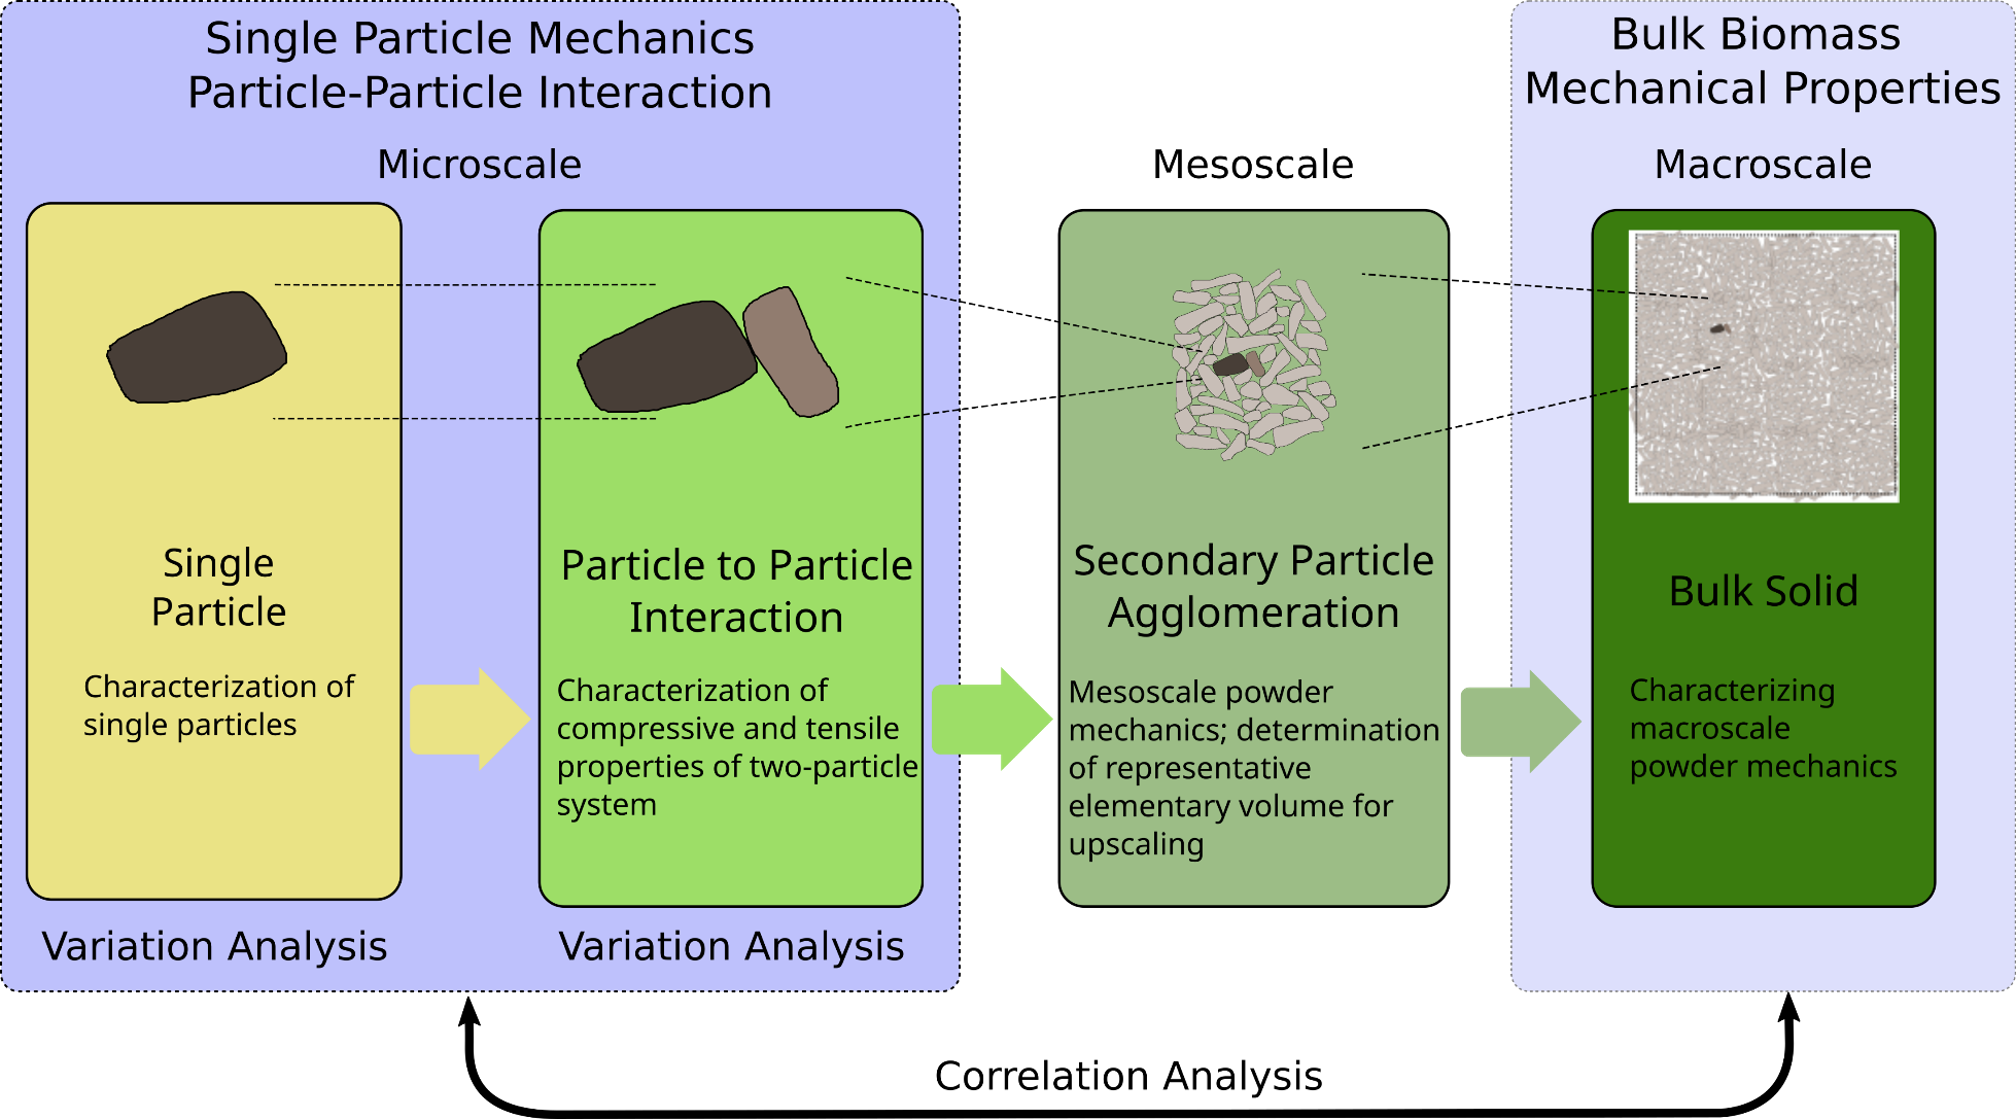
\includegraphics[height=2.75in]{./figures/biomass_multiscale_schematic.png}
\caption{\label{fig:org36c3502}Schematic of the emerging bulk mechanical properties from the mechanical interactions between biomass particles to the bulk mechanical behavior of milled biomass}
\end{figure}

However, the majority of the metrics used for the mentioned flow challenges are focused on bulk behavior and do not address the inter-particle mechanics leading to bulk observation.

\begin{itemize}
\item Janssen's equation \citet{janssen1895versuche} and stresses on silo wall\citet{schulze_examination_1994}
\item Still not quantified Reynolds' question on the relationship between the angle of repose and friction between particles \citet{reynolds_lvii_1885}
\item Recent studies with DEM still relying on fitted parameters that are not determined with particles \citet{xia_defining_2023,chen_hopper_2023,chen_set_2022}
\end{itemize}

Five experimental studies probed friction- and adhesion-related characteristics of milled corn stover.
\begin{itemize}
\item \textcite{fang_friction_2022} : Calibrated friction proxies using repose angle tests on internodal, pith, and nodal tissues.
DEM parameter calibration, repose angle tests, simulation on different tissue types including internodal, pith, nodal tissue
While this study examined angle of repose,
\item \textcite{cheng_effect_2022} : Measured wall friction angles on various surfaces over 0 \(\sim\) 75\% moisture; friction increased with moisture on hydrophilic surfaces but showed non-monotonic behavior on hydrophobic surfaces.
using Experimental, FT4 powder rheometry. comingled bulk milled corn stover measuring flow energy, compressiblity, and wall friction, that are standard test protocols by FT4 powder rheometer.
\item \textcite{leal_impacts_2022} \& \textcite{bose_impacts_2020} : Found biological degradation increases surface energy and work of cohesion for most tissues (stalk, leaf, cob) except cob tissue.
Surface energy/cohesion anatomical fractions of stalk, leaf, and cob using BET, Surface Energy Analyzer, IGC, vOCG and determined surface area, surface energy, wettability, cohesion/adhesion at the bulk scale.

\item \textcite{bose_impacts_2020}  measured  Surface property changes by biological degradation of leaf, stalk, cob using Stereomicroscopy, SEM, and IGC and measured surface roughness, energy, porosity, microbial degradation.

\item \textcite{finney_go_2025} : Magnesium stearate reduces surface energy (up to 40\%) and improves flowability in dry/moderately moist samples.
Examined comingled corn stover using FT power rheometer and IGC and determined flowability, wall friction, surface energy, additive effect, and moisture
\end{itemize}

However, none of the studies provided direct, quantitative measurements of particle-scale friction coefficients or adhesion forces.
Most reported trends or related properties (wall friction angle, surface energy) and qualitative trends.

\textbf{\textbf{Surface Properties and Adhesion}}
\begin{itemize}
\item Leal et al., 2022: Degradation increases surface energy/cohesion except cob. Computed (not measured) adhesion.
\item Bose et al., 2020: Degradation increases aggregation. No direct adhesion measurement.
\item Finney et al., "Go with the Flow": Additive reduces surface energy and improves flow, no direct adhesion numbers.
\end{itemize}

\textbf{\textbf{Moisture Content Effects}}
\begin{itemize}
\item Cheng et al., 2022: Moisture reduces flowability, increases compressibility, raises wall friction (hydrophilic), hydrophobic: non-monotonic.
\item Finney: Mg stearate effective at \(\leq\) 15\% moisture, not above.
\item Leal/Bose: Moisture and degradation increase cohesion/aggregation.
\end{itemize}

\textbf{\textbf{Flow Characteristics}}
\begin{itemize}
\item Fang et al., 2021: Friction coefficients (by tissue type) affect repose angle and flow, validated in simulation.
\item Cheng et al., 2022: 15\% moisture = max flow energy; 75\% = lowest. Increased moisture increases compressibility, reduces flowability.
\item Leal/Bose: Degraded tissues leads to poor flow, agglomeration, arching. Bose: microbial degradation increases aggregation, blockage.
\item Finney: Mg stearate improves flow (dry/15\%), reduces wall friction angle, little effect for high-moisture.
\end{itemize}

In these studies, it was found that misture and surface chemistry are keys to bulk flowability.
However, direct quantitative friction or adhesion values for plant tissues/particles are missing in all studies.
Main handling challenges: friction, agglomeration, arching, rat-holing, surface modification by moisture and degradation-all are repeatedly noted.
Understanding interparticle mechanics associated with each corn stover fraction will provide valuable information for understanding the overall poor flow behavior of milled corn stover.
More specifically, such quantitative information will help identify certain fractions that may be significantly responsible for the poor flowability behavior of comingled corn stover fractions.

There exists a ASTM standards concerning the measuring friction coefficient including \textcite{astmg115-10GuideMeasuringReporting2018}.
However, listed methods in \textcite{astmg115-10GuideMeasuringReporting2018} assumes a specific geometry, e.g., flat surface or sphere, and not feasible to implement for testing milled biomass particles, which are much smaller in size and irregular in shape.
Also test protocols reflects repeated sliding in cyclic motion or rotation, which is implemented in a typical tribometer.
This also reflects specific industrial applications such as ball bearing or sliding frames, which are not applicable to the interactions of biomass particles relevant to the bulk biomass flow.

In other words, the current friction measurements focus on interactions between sliding surfaces, e.g., bearing.
This focus is also reflected in the DEM framework, requiring sliding and rolling friction coefficient.
From the perspective of the handling bulk biomass, or any other cohesive particulate materials, the friction coefficient of incipient relative motion between particle is of interest.

Therefore, we developed an in-house instrument and protocol that can determine mechanical interaction between biomass particles following the Derjaguin's adhesive friction model \citep{gao_frictional_2004,derjaguin1934molekulartheorie,derjaguin_effect_1975}.

This study aims to gain quantitative knowledge of the interparticle mechanics of fractionated corn stover through the development of an interparticle mechanics tester capable of accommodating biomass particles and a test protocol to determine friction and adhesion properties.
With the novel data on interparticle mechanical properties of corn stover particles from different anatomical origins, this study aims to examine the significance of the difference in friction coefficients between corn stover particles from different anatomical fractions.
The knowledge gained by this study will contribute to reducing operational challenges by removing fractions with high friction and traction adhesion contributions.
\subsection{Other notable quotes}
\label{sec:org7f97faf}
\fullcite{kenney_understanding_2013} page 121: Variability of biomass exceeds handling machinery design specification: This paper also mentions about the start-up or continuous running efficiency
\section{Materials and Methods}
\label{sec:org5d422b6}
This section details the method used to determine friction coefficients between anatomical fractions of corn stover.

\begin{figure}[htbp]
\centering
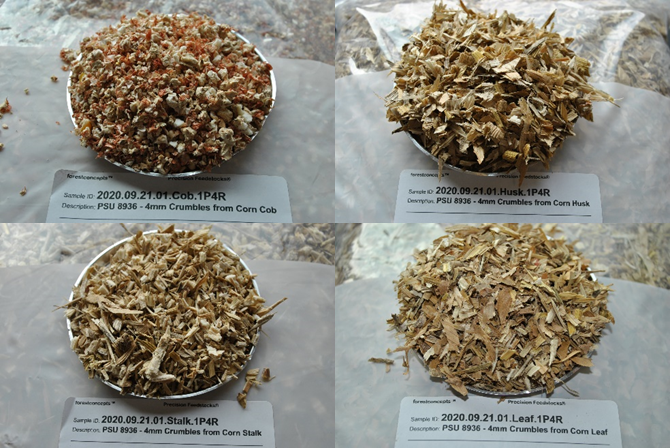
\includegraphics[width=.9\linewidth]{figures/image2.png}
\caption{\label{fig:org7c3c347}Sample images of individual corn stover fractions used in the present study. 4mm cob Crumbles® (top left), 4mm husk Crumbles® (top right), 4mm stalk Crumbles® (bottom left), and 4mm leaf Crumbles® (bottom right)}
\end{figure}
\subsection{Materials}
\label{sec:org22479dd}
A field-dried square bale of corn stover supplied by Antares Corn Stover (Hardin, IA) was manually fractionated into cob, husk, leaf, and stalk tissues.
Each fraction was comminuted to Forest Concepts Crumbles® with a Crumbler® rotary shear (Forest Concepts, Auburn, WA) and
screened on a three-deck orbital classifier to achieve a target geometric mean diameter of 4 mm.
Screen performance was consistent across tissues:
the geometric mean diameter and sphericity differed by \(leq)\) 0.2 mm and \(\leq\) 0.05, respectively (Table \ref{tab:org648519d}).
Despite this size uniformity, loose bulk density varied almost four-fold-from \qty{53}{\kilo\gram\per\cubic\meter} in husk
to \qty{199}{\kilo\gram\per\cubic\meter} in cob, while tapped density followed the same trend (Wilcoxon rank-sum, p < 0.05).

These differences reflect intrinsic anatomical and compositional contrasts among tissues.
Cob tissue is highly lignified \parencite{berchem_corn_2017} and contains closed, pith-filled vascular bundles \parencite{thornburg_mass_2022},
leading to a higher true solid density and more equant particle shapes that pack efficiently.
In contrast, husk and leaf particles are thin, planar, and flexible, creating interlocking voids \parencite{thornburg_mass_2022,li_characterization_2020} that
can lower bulk density and increase compressibility.

\begin{table}[htbp]
\caption{\label{tab:org648519d}Physical properties of corn stover particles of different tissue type (Forest Concepts, LLC analytics laboratory in Auburn, WA). Values after \textpm{} represents standard error.}
\centering
\begin{tabular}{llllll}
\textbf{Anatomical} & \textbf{Moisture} & \textbf{Geometric Mean} &  & \textbf{Bulk Density} & \\
\textbf{Fraction} & \textbf{Content} & \textbf{Diameter (mm)} &  & \textbf{(kg/m\^{}3)} & \\
\hline
 & \emph{\textbf{\%MC wb}} & \emph{\textbf{Xgm}} & \emph{\textbf{Sgm}} & \emph{\textbf{Loose}} & \emph{\textbf{Tapped}}\\
\hline
Cob & 8.9 \textpm{} 3.2 & 6.6 \textpm{} 0.2 & 1.6 \textpm{} 0.0 & 199 \textpm{} 2.4 & 240 \textpm{} 1.5\\
Husk & 7.0 \textpm{} 5.0 & 4.6 \textpm{} 0.2 & 1.6 \textpm{} 0.0 & 53 \textpm{} 2.6 & 72 \textpm{} 0.3\\
Leaf & 7.0 \textpm{} 4.0 & 3.9 \textpm{} 0.2 & 1.6 \textpm{} 0.0 & 56 \textpm{} 3.1 & 74 \textpm{}   3.6\\
Stalk & 8.9 \textpm{} 3.9 & 4.5 \textpm{} 0.0 & 1.8 \textpm{} 0.0 & 84 \textpm{} 0.9 & 109 \textpm{} 0.7\\
\hline
\end{tabular}
\end{table}

Xgm and Sgm of cob and leaf particles are the only statistically different (\(p < 0.05\) from Dunn's test post-hoc) fraction.
Because particle size distributions are similar across tissue types (\(p > 0.05\) from Kruskal\_Wallis test),
the divergent bulk densities indicate true solid density, particle morphology, and packing mechanisms, rather than particle size governed bulk flow behavior.
Lower-density, high-aspect-ratio particles, i.e., husk and leaf, are thought to create large interstitial voids leading to lower bulk density and
exhibit greater compressibility, which is detrimental to mass-flow hoppers and auger feeding systems.
\subsection{Particle size distribution}
\label{sec:orga50c622}

Corn Stover Fractions
Cob shows distinctly different behavior with more material retained at larger sizes (4.75-5 mm) compared to other fractions1
Husk, leaf, stalk, and comingled fractions show similar PSD patterns with steep curves between 2-4 mm1
Most material across all fractions is retained between 2-5 mm opening sizes1
Southern Pine Residue Fractions
Needle fraction shows significantly different behavior with most material passing through larger openings until 2.5 mm1
Bark, chip, and twig fractions exhibit similar PSD patterns1
More uniform distribution across different size ranges compared to corn stover1
Implications
Processing Efficiency
The different PSD patterns between fractions suggest that separate processing conditions might be optimal for different plant parts
Cob (corn stover) and needle (pine) fractions may require different handling strategies due to their distinct size distributions
Material Properties
The differences in PSD reflect the inherent structural differences between:
Woody biomass (pine residue) with more rigid fiber structure
Herbaceous biomass (corn stover) with more flexible fiber arrangement
Downstream Applications
The varying particle size distributions could affect:
Bulk density and flowability in storage and handling
Surface area available for biological or chemical conversion
Heat and mass transfer in thermochemical conversion processes
This understanding can help optimize processing parameters and downstream conversion processes for different biomass fractions.


Corn Stover Fractions
Cob shows distinctly different behavior with more material retained at larger sizes (4.75-5 mm) compared to other fractions1
Husk, leaf, stalk, and comingled fractions show similar PSD patterns with steep curves between 2-4 mm1
Most material across all fractions is retained between 2-5 mm opening sizes1
Southern Pine Residue Fractions
Needle fraction shows significantly different behavior with most material passing through larger openings until 2.5 mm1
Bark, chip, and twig fractions exhibit similar PSD patterns1
More uniform distribution across different size ranges compared to corn stover1
Implications
Processing Efficiency
The different PSD patterns between fractions suggest that separate processing conditions might be optimal for different plant parts
Cob (corn stover) and needle (pine) fractions may require different handling strategies due to their distinct size distributions
Material Properties
The differences in PSD reflect the inherent structural differences between:
Woody biomass (pine residue) with more rigid fiber structure
Herbaceous biomass (corn stover) with more flexible fiber arrangement
Downstream Applications
The varying particle size distributions could affect:
Bulk density and flowability in storage and handling
Surface area available for biological or chemical conversion
Heat and mass transfer in thermochemical conversion processes
This understanding can help optimize processing parameters and downstream conversion processes for different biomass fractions.
\subsection{Inter-particle Mechanics (IPM) Tester}
\label{sec:orga00b64d}
Existing tribometer, similar to the instrument used in \citet{chen_measurements_2020},
is challenging to be used in determining friction coefficient of milled biomass particles.
unless employing an additional attachment due to the dimension of typical milled biomass particles.
In addition, the cyclic reciprocating movement is not simulating the frictional interaction between biomass particles during handling,
while it is thought to be an adhesive friction following Derjaguin's law \citep{derjaguin_influence_1994,derjaguin1934molekulartheorie}.

To overcome such shortfalls, we developed a new Inter-particle Mechanics (IPM) (Figure \ref{fig:orgeb709cb}) to measure the traction force between a stationary and moving particle under a varying magnitude of normal load.
This arrangement allows for one test run to produce multiple normal force and lateral force measurements and alleviates the requirement to conduct separate tests with different normal forces in a conventional friction tester \citep[][astmg115-10GuideMeasuringReporting2018]{pitenis_leonardo_2014}.
The development of the new design was essential for simulating any possible orientation of two interacting particles.
This design allows collecting friction coefficients over multiple untested regions without resampling surfaces or replacing test particles between each repetition.
With this design, it is also possible to prepare and condition multiple test samples, e.g., conduct friction experiments in an environment-controlled chamber at a different environmental relative humidity.

\begin{figure}[htbp]
\centering
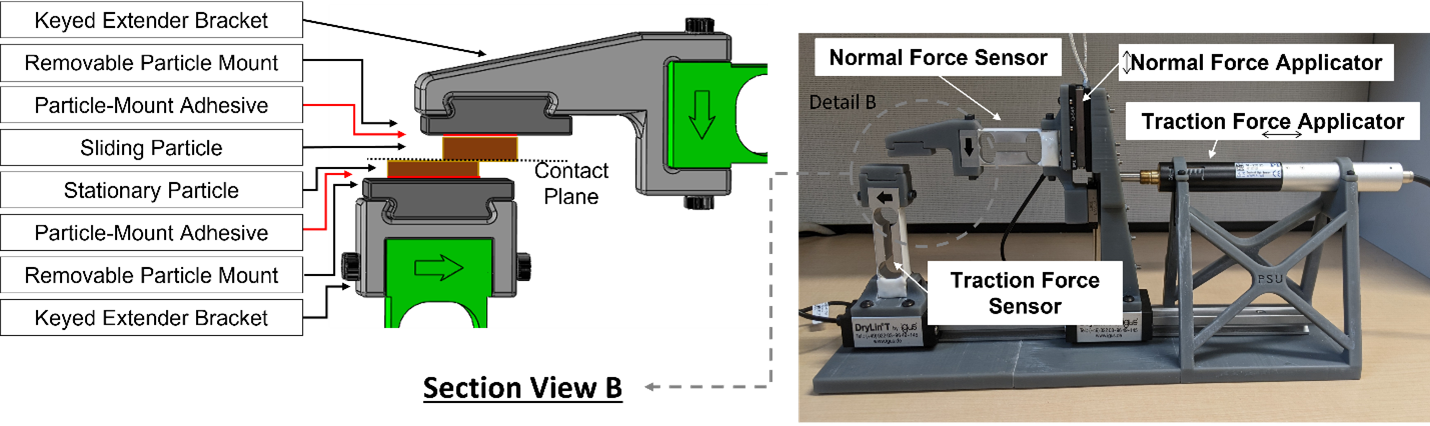
\includegraphics[width=.9\linewidth]{figures/image3.png}
\caption{\label{fig:orgeb709cb}Inter-particle mechanics tester (right) with a detailed view of sample mounting (left).}
\end{figure}
\subsection{Specifications and Operational Parameters of Interparticle Mechanics Tester}
\label{sec:orgde26a81}
The designed Inter-Particle Mechanics Tester (IPMT, \parencite{slosson_characterization_2025}) can to perform friction tests on fully supported particles, unsupported (over-hanging), or combinations of both.
Sample holders and component position and capacity are easily adjustable to handle particles of any size and shape.
Considering the need to characterize the frictional contact with the perspective of storage and incipient flow of milled biomass,
IPMT was designed to have a minimum incremental push and pull motion of \qty{0.05}{\micro\meter},
and a typical push and pull velocity is set to \qty{1.2}{\milli\meter\per\second}, which can be modified.
To accommodate a typical biomass particle dimension,
the maximum push and pull travel ranges up to \qty{25}{\milli\meter} to accommodate a typical biomass particle size.
For vertical direction movement, the maximum displacement of the normal force actuator is \qty{14}{\milli\meter} to accommodate a typical biomass particle size.
The resolution of the both actuators are \qty{6}{\nano\meter}.
Combined vertical and lateral displacement actuators make it possible to control the initial particle contact location if there exists a specific region of interest. The maximum forces of vertical and normal force censors are \qty{20.02}{\newton} and \qty{2.94}{\newton}, respectively,
with the accuracy of \qty{\pm 0.02}{\percent} of the full scale.
Normal and traction force data were collected at \qty{80}{\hertz}, using National Instruments\textsuperscript{TM} LabVIEW (Version 2022, Austin TX) and
two 24-bit Di-1000U signal digitizers (Loadstar Sensors, Freemont, CA).
\subsection{Experimental Design and Setup}
\label{sec:orge48fec6}
An experimental procedure was developed to perform friction tests with minimal experimental error.
A sample size of 15 was selected for each possible combination of anatomical fractions to ensure the quality of a subsequent analysis of variance (Kruskal-Wallis test with \(\alpha=0.05\)).
The Wilcoxon signed-rank (signed-rank) test was conducted to test the null hypotheses,
i.e., friction coefficients and adhesion forces between corn stover particles from different anatomical fractions are not statistically different,
without assuming a statistical distribution of determined friction coefficient and adhesion forces.
To prepare an inter-particle mechanics test, approximately \qty{50}{\gram} samples were collected from each anatomical fraction of milled corn stover.
Each sample was held in a controlled environment for 72 hours to allow for particles to reach an equilibrium moisture content at approximately \qty{23}{\celsius} and \qty{40}{\percent} relative humidity.
The resulting moisture contents of cob, husk, leaf, and stalk are \qty{8.9(1.0)}{\percent}, \qty{7.0(1.4)}{\percent}, \qty{7.0(1.2)}{\percent}, and \qty{8.9(1.1)}{\percent}, respectively (values after \(\pm\) represent the standard error with n = 11).

Once particle moisture was equalized, particles were randomly selected and adhered to removable particle mounts (Figure \ref{fig:org531e427}) using Ultra Bond\textsuperscript{TM} Super Glue (Permatex Inc.).
Conservative volumes of adhesives were applied to minimize the absorption into particles and ensure proper curing.
From the visual inspection, it appeared that no glue sips into the particle samples,
which is attributed to the high viscosity of the chosen glue and quick initial curing time.
A curing period of longer than 24 hours (\(\pm 2\) hour) was established for experimental consistency.
The curing environment is identical to the moisture-equilibrating environment.
Finally, the grain orientations were randomly chosen with every particle.

\begin{figure}[htbp]
\centering
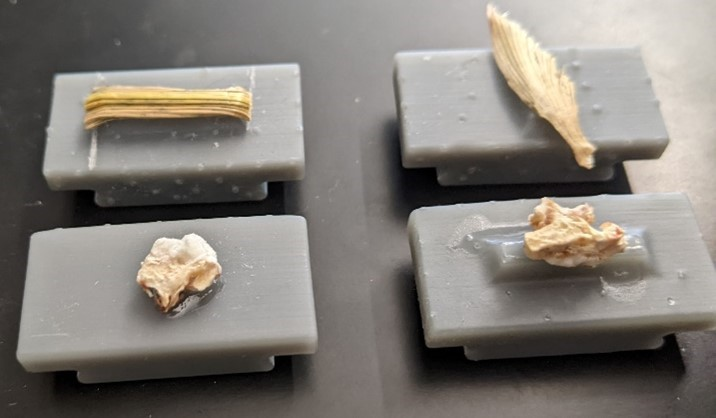
\includegraphics[width=.9\linewidth]{figures/image4.jpg}
\caption{\label{fig:org531e427}Image of corn stover particles adhered to plastic particle mount for conditioning and testing. The upper and lower half of the image contains 4mm husk and cob fractions, respectively.}
\end{figure}

Once the adhesive had cured, particle pairs were randomly selected for testing.
Table \ref{tab:org3d9ce72} lists the combinations of milled corn particles of different tissue types and conducted a number of repetitions for statistical analysis with the chosen significance level (\(\alpha = 0.05\)) to ensure the repeatability.

\begin{table}[htbp]
\caption{\label{tab:org3d9ce72}Experimental plan for the required number of corn fraction test pairs and associated repetitions.}
\centering
\begin{tabular}{ccc}
\hline
\textbf{Base} & \textbf{Interacting} & \textbf{Repetitions}\\
\textbf{Particle} & \textbf{Particle} & \\
\hline
Cob & Cob & 15\\
Cob & Husk & 15\\
Cob & Leaf & 15\\
Cob & Stalk & 15\\
Husk & Husk & 15\\
Husk & Leaf & 15\\
Husk & Stalk & 15\\
Leaf & Leaf & 15\\
Leaf & Stalk & 15\\
Stalk & Stalk & 15\\
\hline
\end{tabular}
\end{table}

An inter-particle mechanics test started with establishing contact between particle samples indicated by a positive normal force reading typically ranging between \qty{0.3}{\newton} and \qty{2}{\newton}.
Then, the lateral sliding was initiated at a speed of \qty{0.5}{\milli\meter\per\minute}.
The normal and lateral forces were tracked and recorded simultaneously until the contact between two particles was lost,
which resulted in a sudden change in the measured force.
The middle two quantifies were selected and extracted as steady-state frictional interaction data for further analysis and the determination of friction coefficient and adhesion force.

To determine the cohesive frictional contact, a modified Amonton's equation by Derjaguin \parencite{derjaguin1934molekulartheorie,gao_frictional_2004,derjaguin_effect_1975}, as defined in the Equation \eqref{eq:Derjaguin_1934}, was used.

\begin{equation}
\label{eq:Derjaguin_1934}
F_{\text{traction}} = F_{0} + \mu\cdot F_{\text{normal}}
\end{equation}
,where \(F_{\text{traction}}\) is the tractional force in the lateral direction,
\(F_0\) is the adhesion force,
\(\mu\) is the coefficient of friction, and
\(F_{\text{normal}}\)  is the normal force representing the contact force.
From this linear relationship, the coefficient of friction (\(\mu\)) was determined from the slope of the best-fit line,
and the adhesion force (\(F_0\)) was determined from the intercept of the best-fit line on the y-axis, i.e., the traction force axis.
For this purpose, linear regression analyses were conducted to determine the coefficient of friction (\(\mu\)) and adhesion force (\(F_0\)) from experimental data.
\section{Results and Discussion}
\label{sec:org59b1bca}
\subsection{Validation of the IPM}
\label{sec:org33a26c4}
To validate the developed Inter-Particle Mechanics tester, a polypropylene sheet was used as a reference material.
A polypropylene sheet with \qty{1.588}{\milli\meter} (1/16 inch) thickness was obtained from McMaster-Carr Supply Company,
which lists the friction coefficient to range from 0.25 to 0.28 based on the specification of the manufacturer.
20 samples were prepared and subjected to the IPM test.
The obtained 20 test results of frictional interaction between two polypropylene sheet samples are shown in Figure \ref{fig:orgf7bd77f},
which clearly shows a linear relationship between normal force and traction force with detectable traction force.
It should be noted that a test commenced with a positive normal force and it is maintained through entire test conducted by tractional movement.
This test procedure resulted in consistent non-zero positive normal force measurements.

\begin{figure}[htbp]
\centering
\includegraphics[height=2.75in]{./figures/figure06_pp_ipm_raw_measurements.png}
\caption{\label{fig:orgf7bd77f}Validation test results of polyprophylene}
\end{figure}

Using Derjaguin's adhesive contact model,
the coefficient of friction and adhesion force were determined from the slope and intercept of the obtained linear relationship through the linear regression analysis. The summary of the determined friction coefficient (\(\mu\)) and adhesion force (\(c\)) are listed in Table \ref{orgbb51f29} and shown in Figure \ref{fig:org422bfc7}.
The determined \(\mu\) and \(c\) values are consistent but smaller than the above-mentioned vendor specification.
The determined friction coefficient is smaller than the listed range.
This is an expected trend because the friction coefficient is reported to be smaller with the smaller normal force and initial sliding friction segment for polypropylene \parencite{gracias_continuum_1998,sedlak_effect_2017}.
This observation supports the accuracy of the Interparticle Mechanics Tester in determining frictional characteristics.

Table \ref{orgbb51f29} lists the results of the validation experiment.

\begin{table}
  \begingroup\footnotesize
  \begin{longtable}{lrrrrrrrrrr}
    \textbf{Variable} & $\mathbf{n}$ & \textbf{Min} & $\mathbf{q_1}$ & $\mathbf{\widetilde{x}}$ & $\mathbf{\bar{x}}$ & $\mathbf{q_3}$ & \textbf{Max} & $\mathbf{s}$ & \textbf{IQR} & \textbf{\#NA} \\
    \hline
    mu & 20 &  0.194 & 0.221 & 0.250 & 0.258 & 0.288 & 0.394 & 0.051 & 0.067 & 0 \\
    c & 20 & -8.472 & 2.048 & 3.790 & 3.309 & 5.488 & 8.931 & 3.657 & 3.441 & 0 \\
    \hline
  \end{longtable}
  \endgroup
\caption{\label{orgbb51f29}Validation test results of polypropylene}
\end{table}

\begin{figure}[htbp]
\centering
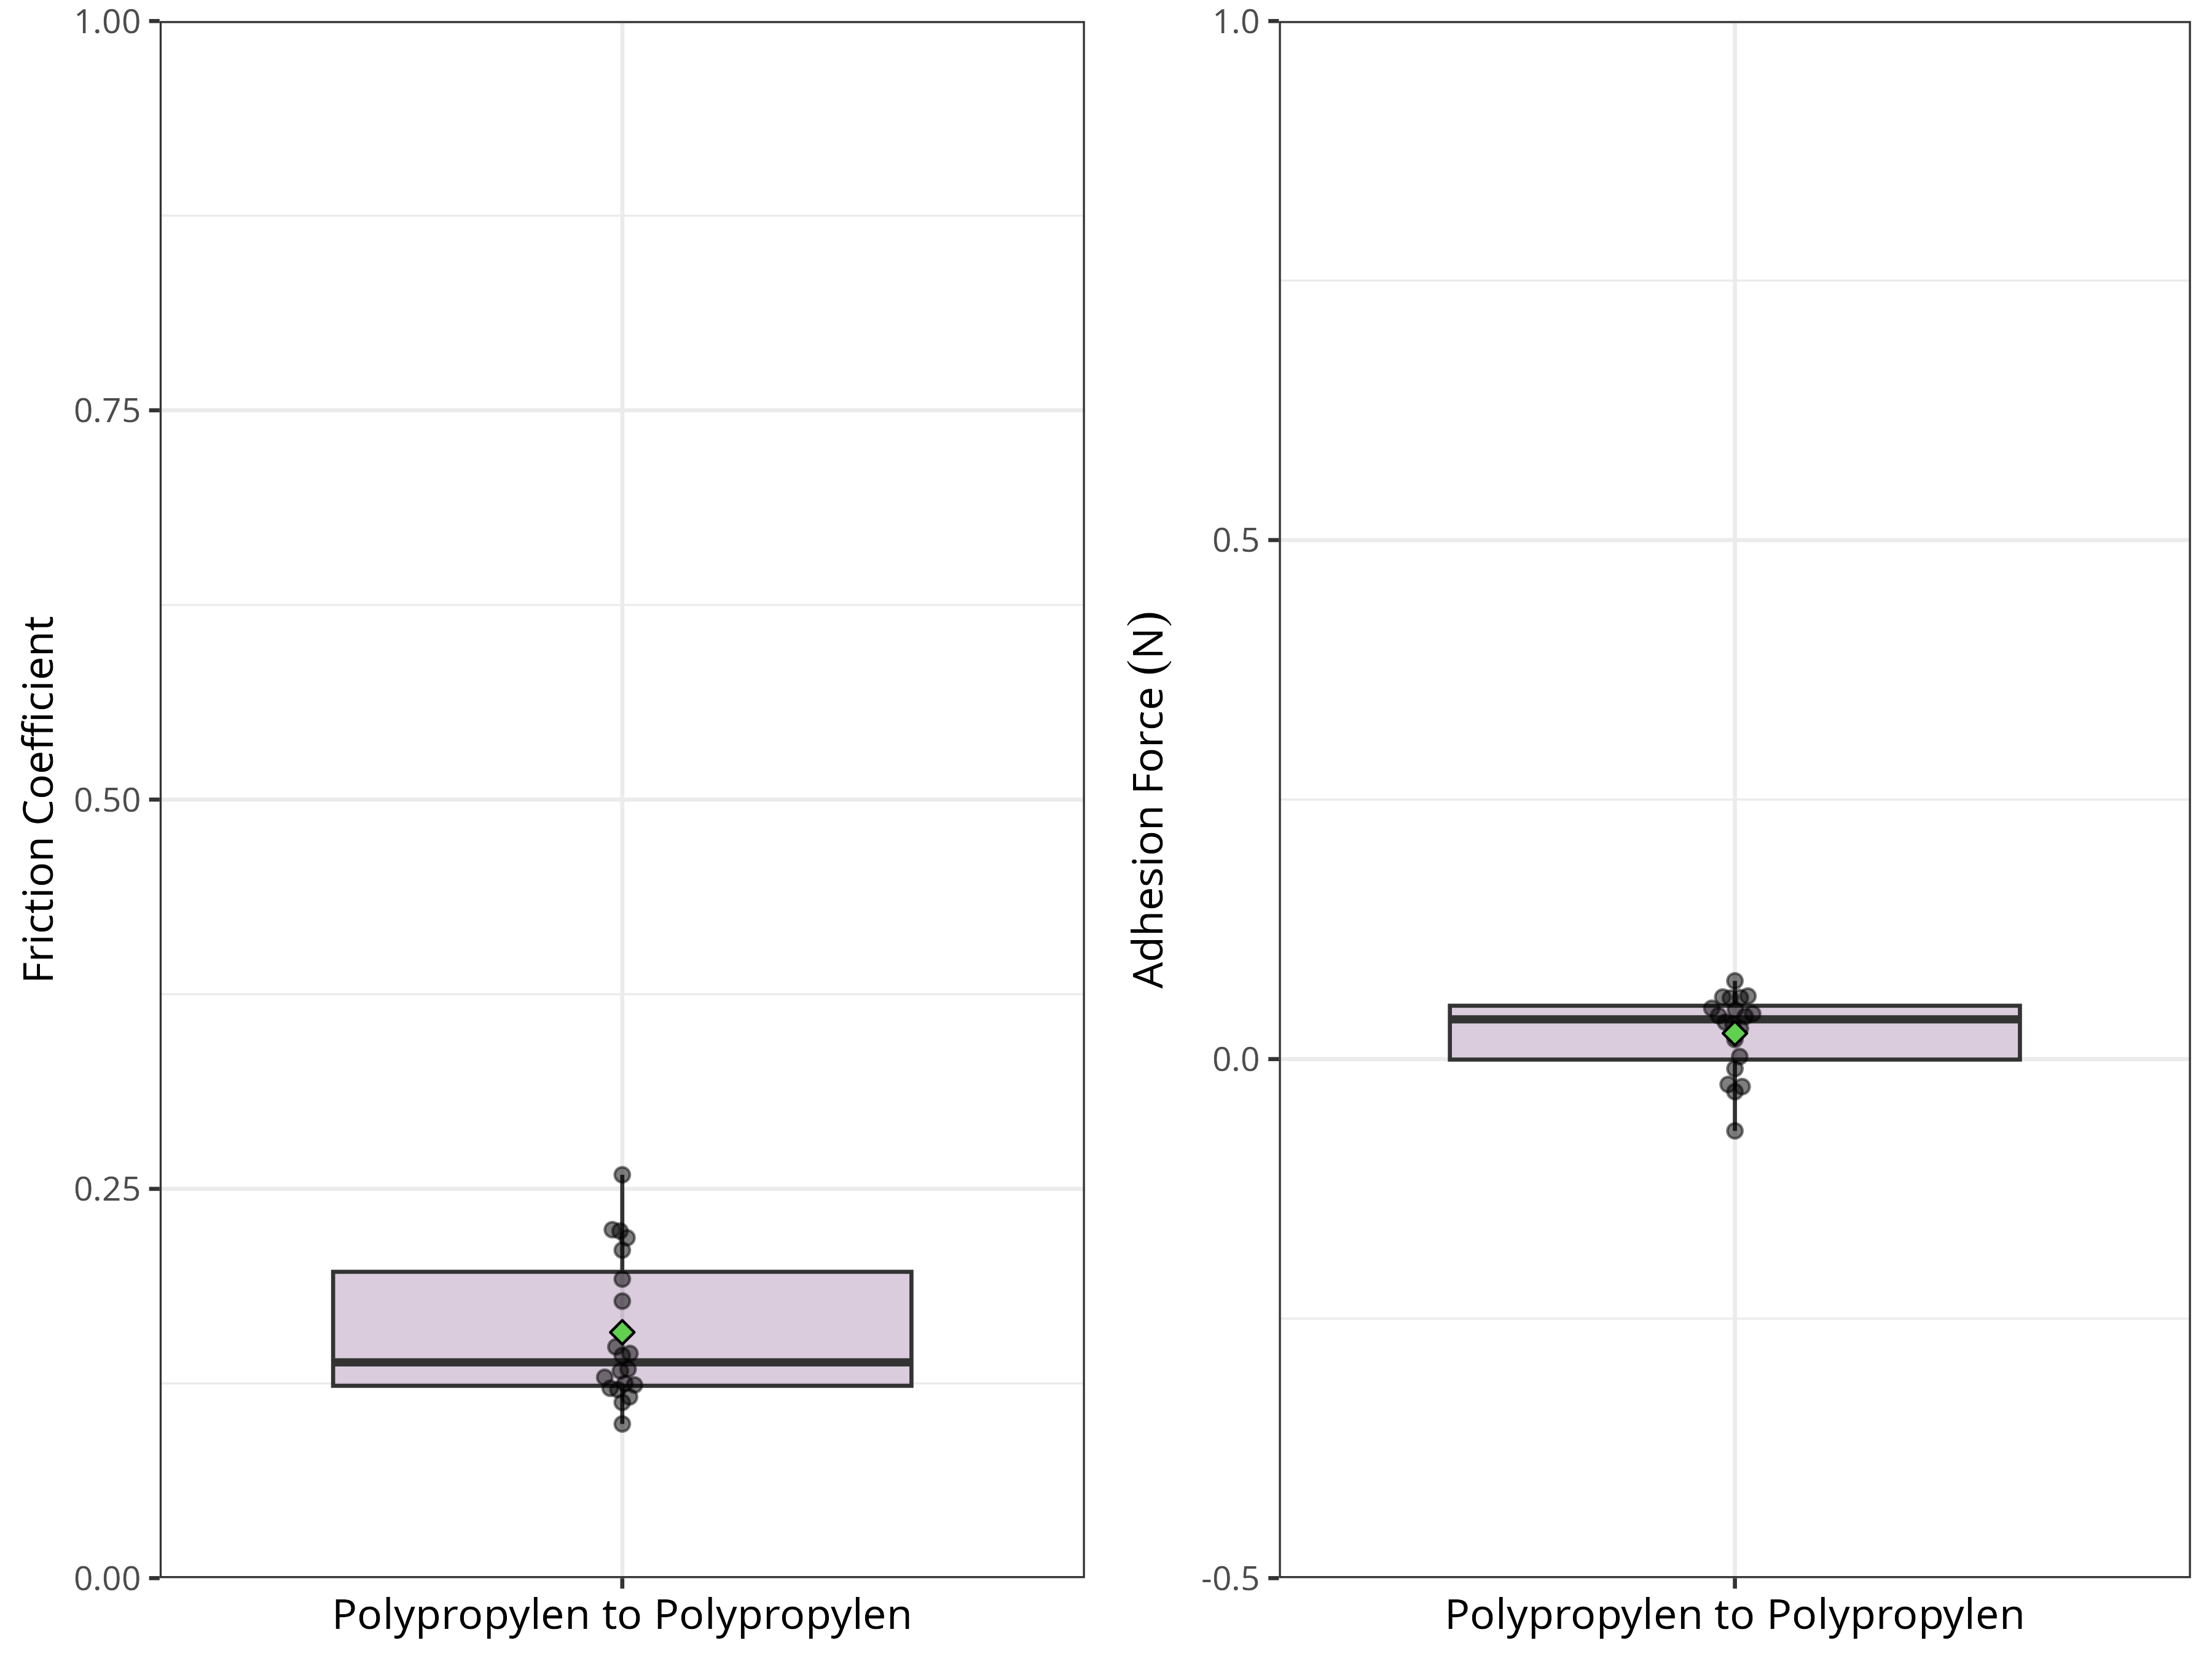
\includegraphics[height=4in]{./figures/pp_pp_comb_ipm_coeffs_box_plts.png}
\caption{\label{fig:org422bfc7}Interparticle Mechanics Test results of polypropylene sheet samples. Each color represents a different run of the experiments (n=20)}
\end{figure}

\newpage
\subsection{Typical corn stover particles IPM results}
\label{sec:org4e7ff97}
\begin{figure}[!htb]
\centering
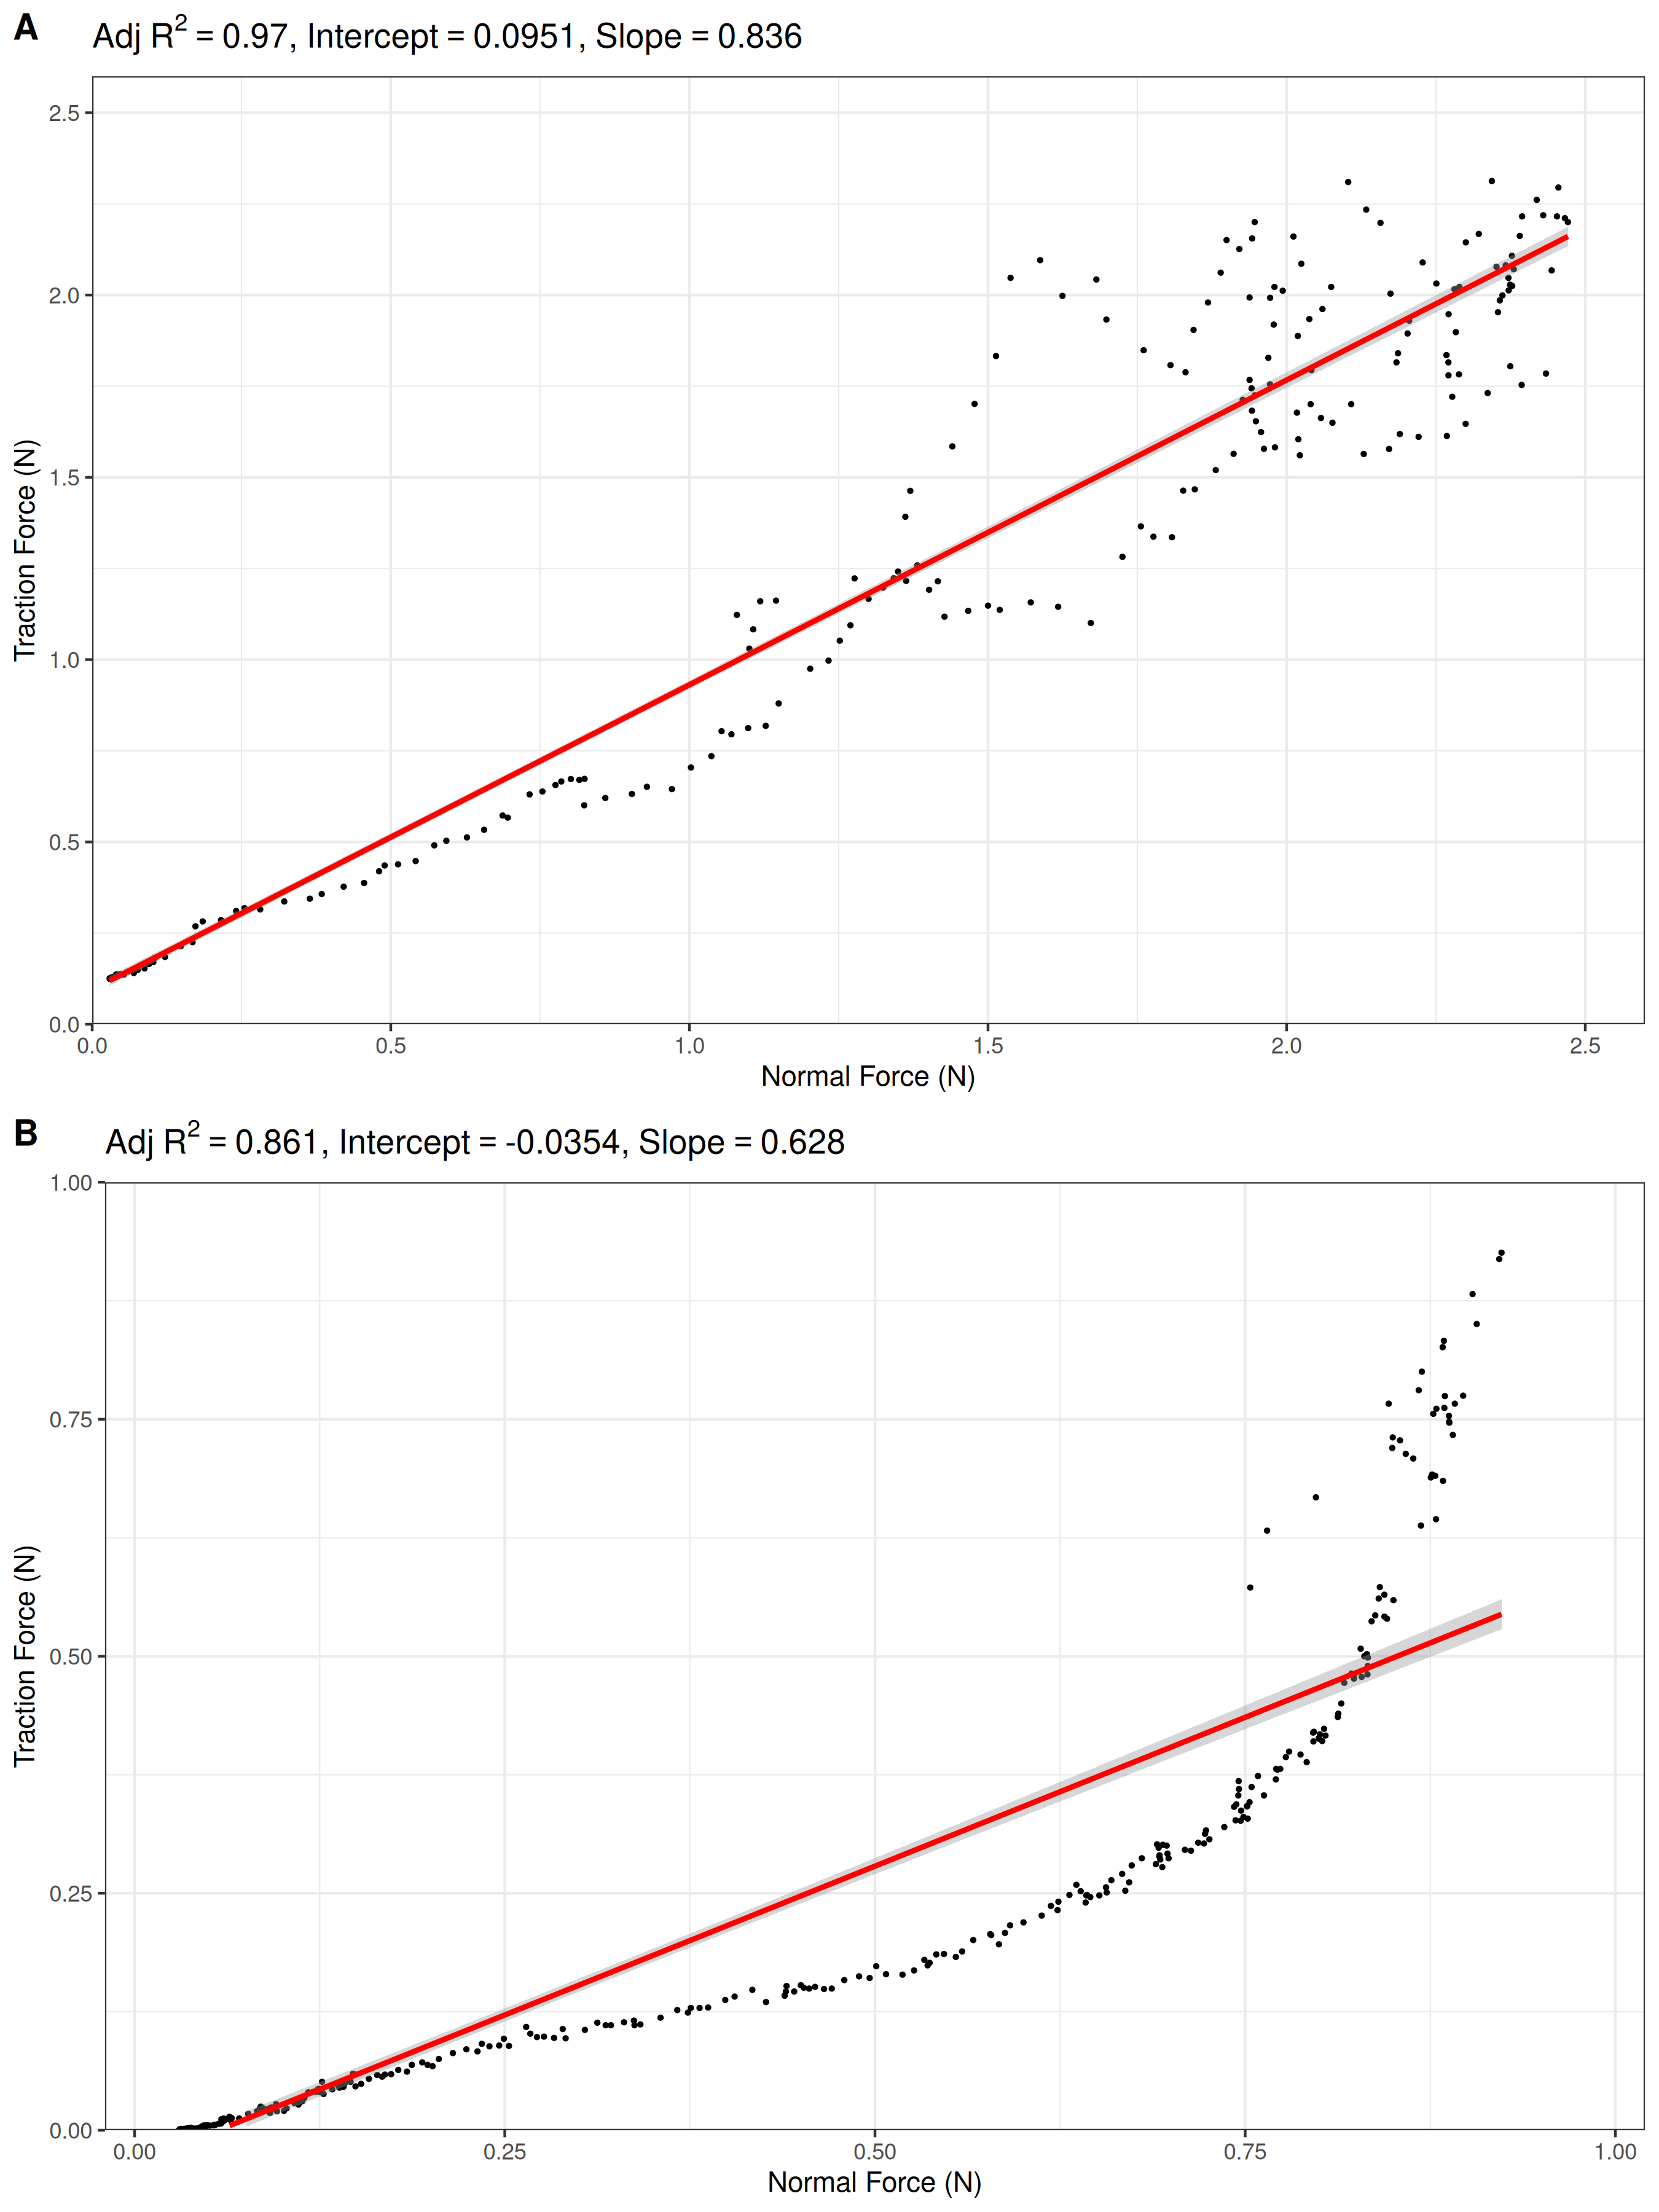
\includegraphics[width=.9\linewidth]{./figures/typical_result_cs_two_cases.png}
\caption{\label{fig:org6570482}Typical corn stover particle result (A is from cob particle vs. cob particle and B is from cob particle vs stalk particle)}
\end{figure}


To examine the variability in frictional contact mechanics between corn stover particles from different tissue types, corn stover samples were manually fractionated into the cob, husk, leaf, and stalk, then crumbled using a 4 mm screen using Crumbler\textsuperscript{\textregistered} by Forest Concepts, LLC. Twenty particle sample pairs for each tissue type were prepared, and the interparticle mechanics tests were conducted. A typical experimental data and regression analysis result is shown in Figure \ref{fig:org6570482}. \marginnote{may want to use different result for dt\_ad\_cs typical\_stalk\_stalk 20230505\_11 plt}
It is notable that normal force approaches to zero value when compared to the polypropylene validation test (Figure \ref{fig:org6570482}).
Zero traction force with zero normal force is thought to occur because of highly uneven surface of biomass particle.
In other words, while such rough surface can increase frictional resistance to traction sliding, but
lateral movement can also reduce the required force to maintain the movement.
This observation poses an interesting problem in describing cohesive friction interaction between biomass particles, which is discussed in detail below.

Derjaguin's linear model and other polynomial models reflecting the observation of \textcite{sedlak_effect_2017} hinting that friction coefficient values can be smaller when the applied normal force is smaller.
\newpage
\subsection{Friction coefficient and Adhesion forces between corn stover particles from the same tissue type}
\label{sec:orgd65e16c}
\begin{figure}[htbp]
\centering
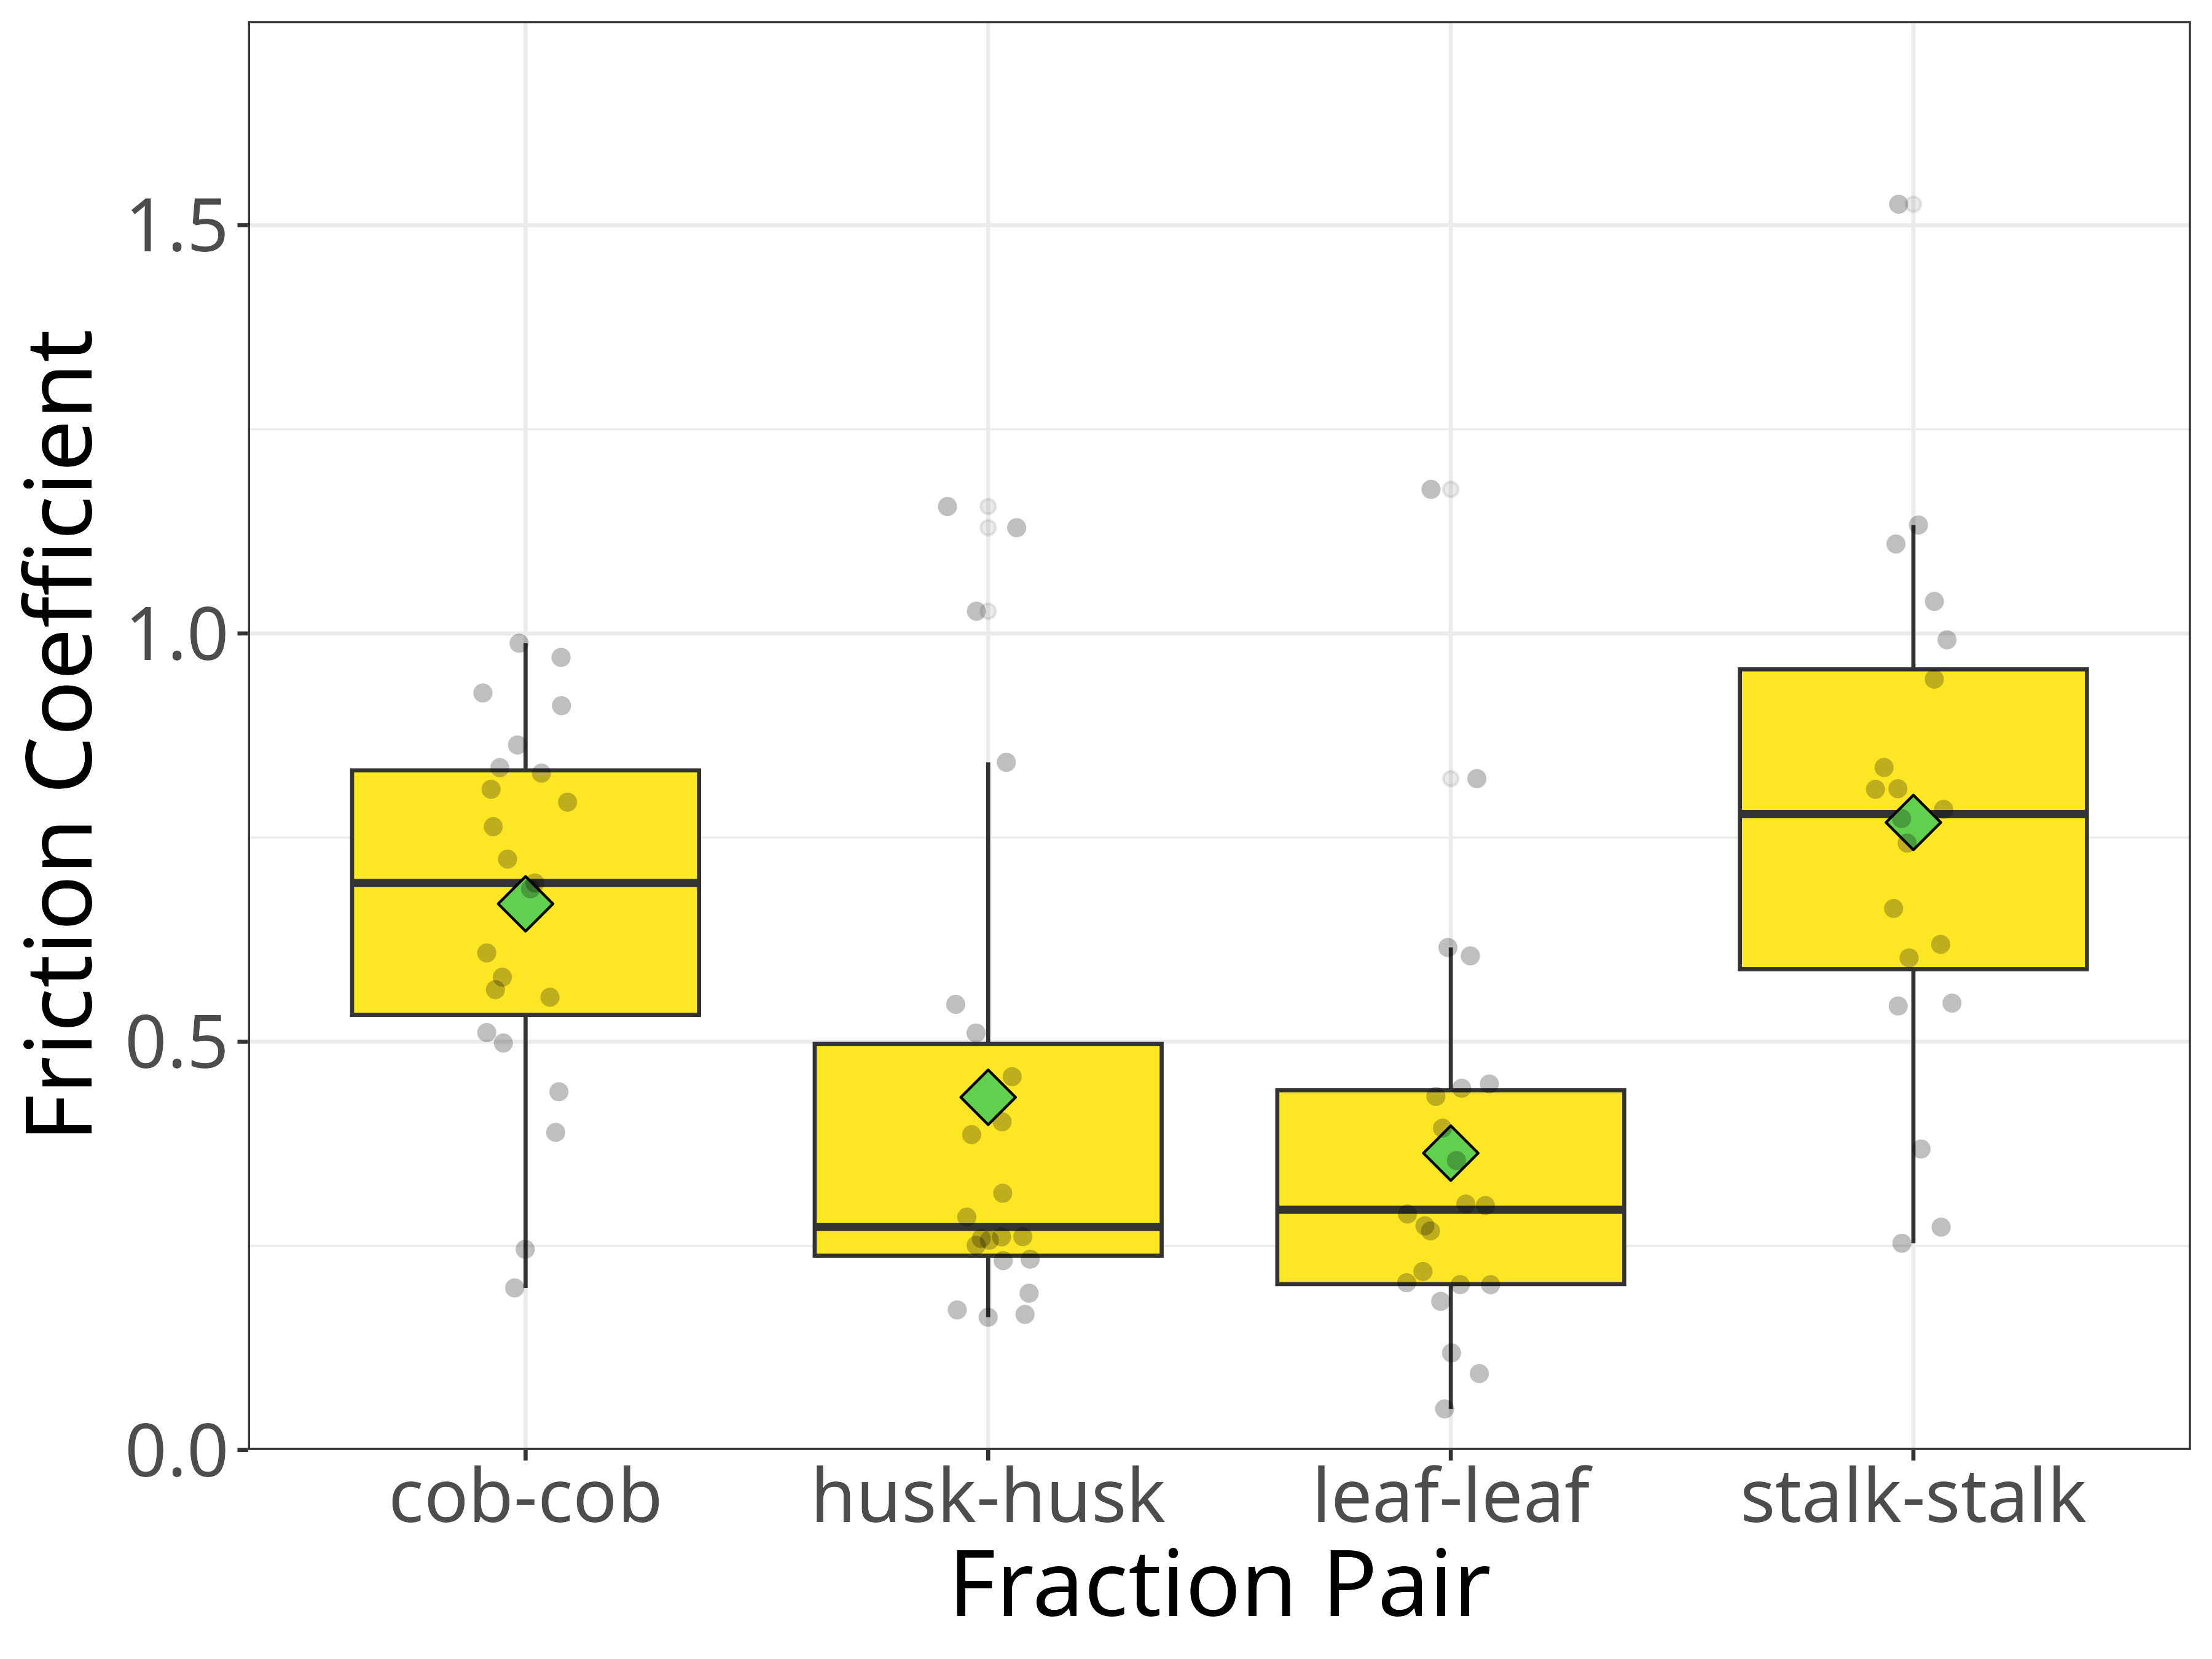
\includegraphics[height=4in]{./figures/cs_cs_same_fraction_coeff_mu_box_plt.png}
\caption{\label{fig:org2ba45ee}Friction coefficient between corn stover particles of same tissue type}
\end{figure}

\newpage

\begin{figure}[htbp]
\centering
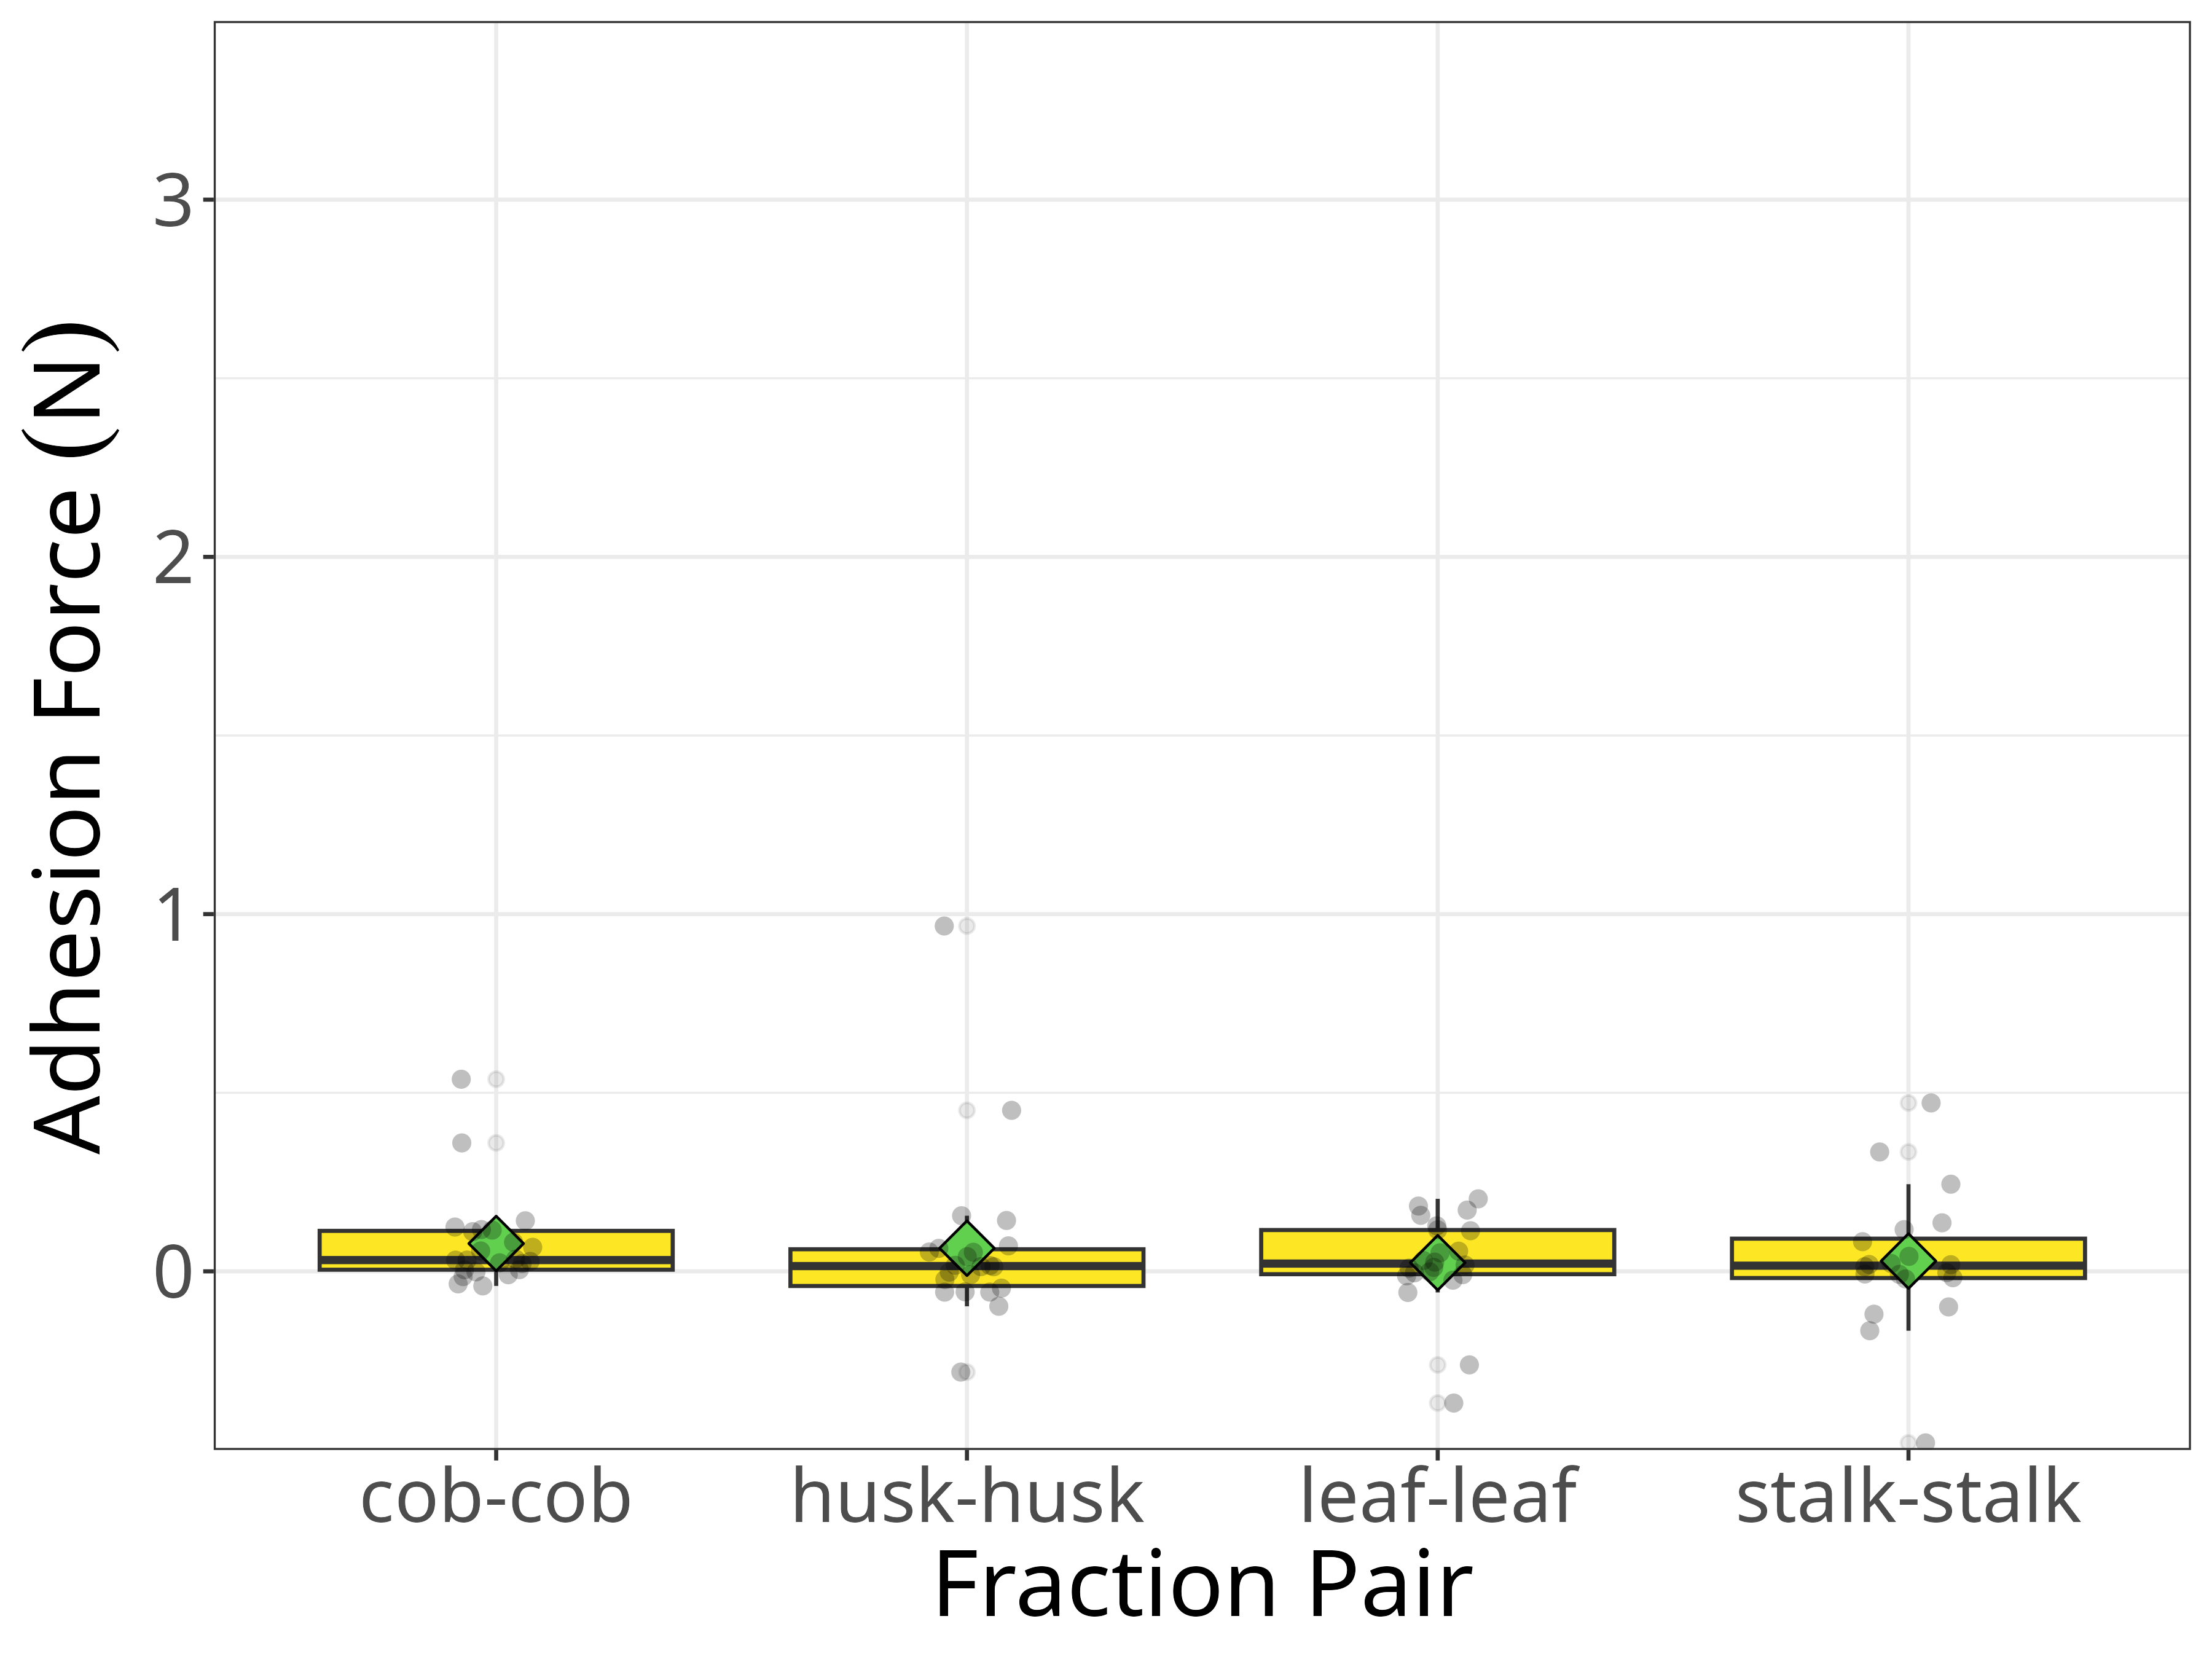
\includegraphics[height=4in]{./figures/cs_cs_same_fraction_coeff_c_box_plt.png}
\caption{\label{fig:org2603551}Adhesion force between corn stover particles of same tissue type}
\end{figure}


The determined friction coefficient and adhesion forces of corn stover particles are shown in Figure \ref{fig:org2ba45ee} and Figure \ref{fig:org2603551}.
The analysis of corn stover particle interactions reveals distinct patterns in both friction coefficients and adhesion forces across different fraction pairs. Among the friction coefficients, cob-cob and stalk-cob interactions demonstrate the highest values at 0.636 and 0.629 respectively, indicating substantial frictional resistance between these particle types. The moderate friction range includes husk-cob and stalk-husk combinations, showing coefficients of 0.464 and 0.437, while stalk-stalk interactions exhibit intermediate friction behavior with a coefficient of 0.483.

Leaf-based interactions consistently display lower friction coefficients, with leaf-leaf pairs showing 0.255, leaf-husk pairs at 0.275, and leaf-cob combinations reaching 0.445. This pattern suggests that leaf material generally creates less frictional resistance compared to other corn stover components.

Regarding adhesion forces, all fraction pairs exhibit negative values, indicating repulsive forces between particles.
This observation indicates that when two biomass particles are contacting each other with less than a couple of Newtons (100 gf or less),
it will make each particles displaced away from each other.
Depending on the direction of such relative motion, this phenomenon can help the bulk flow in the gravity direction or hinder the initiation of flow.
At higher normal force (\(\gamma\times h\), where \(\gamma\) is bulk density and \(h\) is height of the bulk) condition,
the observed small adhesion force can be interpreted as cohesive interaction.
This observation alludes the complex problem of the incipient flow of the bulk.
On the other hand, for the particles in motion, the normal force between particles can be thought to be minuscule, which will make the contact cohesionless.

Stalk-stalk pairs demonstrate the strongest adhesion with a value of -0.074, closely followed by husk-husk interactions at -0.071.
Stalk-cob and leaf-husk pairs show moderate adhesion forces around -0.060, with husk-cob interactions similarly positioned at -0.057.
An interesting inverse relationship emerges between friction and adhesion properties. Notably, cob-cob interactions show the lowest adhesion force at -0.027 despite having high friction, while stalk-leaf and stalk-husk pairs demonstrate relatively lower adhesion forces around -0.043. This pattern suggests that materials with high friction coefficients tend to exhibit lower adhesion forces, while those with strong adhesion generally show moderate friction coefficients. Leaf-based interactions maintain their unique character by consistently showing lower friction coefficients paired with moderate to high adhesion forces.
\begin{itemize}
\item summary observations
\label{sec:orgf08c9a6}
\begingroup\footnotesize
The mechanical properties of agricultural residues, particularly corn stover, are critical parameters in the design and optimization of biomass processing systems. Understanding the frictional interactions between particles of different tissue types provides fundamental insights into powder mechanics behavior, flow characteristics, and processing efficiency. This investigation focuses exclusively on homogeneous tissue interactions to isolate the intrinsic mechanical properties of individual corn stover components.
\begin{itemize}
\item Results and Discussion
\label{sec:org14c0a6a}
\begin{itemize}
\item Friction Coefficient Analysis \newline
\label{sec:org37a7087}
The analysis of homogeneous tissue interactions revealed distinct frictional characteristics across the four corn stover tissue types. Cob particles exhibited the highest mean friction coefficient (\(\mu = 0.669 \pm 0.221\)), followed by stalk (\(\mu = 0.515 \pm 0.786\)) husk (\(\mu = 0.392 \pm 0.331\), and leaf tissues (\(0.342 \pm 0.274\)).
\item Friction coefficient and adhesion force distributions for corn stover tissue homogeneous interactions \newline
\label{sec:orgaa59af3}
The coefficient of variation analysis demonstrated considerable heterogeneity within tissue types, with stalk particles showing the highest variability (CV = 152.5\%) and cob particles exhibiting the most consistent behavior (CV = 33.1\%). This variability pattern suggests that stalk tissues possess more heterogeneous surface properties, potentially due to the complex vascular structure and varying lignification patterns within this tissue type.
\item Adhesion Force Characteristics \newline
\label{sec:org05afe1e}
Adhesion forces followed a different ranking pattern compared to friction coefficients. Cob particles demonstrated the highest mean adhesion force (\(c = 0.078 \pm 0.131\)), followed by husk (\(c= 0.068 \pm 0.231\), stalk (\(c = 0.064 \pm 0.221)\)), and leaf tissues (\(c = 0.024 \pm 0.131\)).
The relatively low magnitude of adhesion forces across all tissue types indicates weak cohesive interactions,
consistent with the dry agricultural residue nature of corn stover.
\item Statistical Significance and Distribution Patterns \newline
\label{sec:org7cd9cca}
One-way ANOVA analysis revealed that while differences in friction coefficients approached statistical significance (\(F = 2.280, p = 0.085\)),
adhesion forces showed no significant inter-tissue variation (\(F = 0.380, p = 0.768\)).
This finding suggests that friction coefficients are more discriminative parameters for characterizing tissue-specific mechanical properties.
\item Distribution analysis revealed notable skewness patterns across tissue types: \newline
\label{sec:orgeef3fdb}
Stalk particles exhibited strong negative skewness in friction coefficient distribution (skewness = -2.733), indicating the presence of low-friction outliers, while husk and leaf tissues showed positive skewness (1.183 and 1.261, respectively). These distribution characteristics reflect the inherent structural complexity and surface heterogeneity of different corn stover components.
\item Correlation Analysis and Mechanical Coupling \newline
\label{sec:org9573ea2}
The correlation between friction coefficient and adhesion force varied significantly among tissue types. Leaf particles showed the strongest negative correlation (r = -0.395), suggesting an inverse relationship between surface roughness and cohesive forces. Conversely, husk particles exhibited a positive correlation (r = 0.311), indicating potential coupling between frictional and adhesive mechanisms. Cob and stalk tissues showed weak correlations (r = -0.201 and -0.033, respectively), suggesting independent friction and adhesion mechanisms.
\item Implications for Powder Mechanics \newline
\label{sec:org7d78d31}
The observed tissue-specific variations have significant implications for corn stover processing systems. The higher friction coefficients observed in cob particles suggest increased energy requirements for size reduction and handling operations. The high variability in stalk particle properties indicates the need for adaptive processing strategies to accommodate the heterogeneous nature of this tissue type.

The relatively low adhesion forces across all tissue types suggest that corn stover particles exhibit free-flowing characteristics under dry conditions, which is advantageous for bulk handling and storage applications. However, the tissue-specific differences may lead to segregation phenomena in mixed-tissue systems.
\item Materials and Methods \newline
\label{sec:org0218db5}
The experimental dataset comprised 94 measurements of homogeneous tissue interactions (cob-cob: n=23, stalk-stalk: n=24, husk-husk: n=24, leaf-leaf: n=23) conducted on 4mm corn stover particles. Friction coefficients and adhesion forces were determined using Dejaguin's cohesive friction relationship. Statistical analysis included descriptive statistics, ANOVA, correlation analysis, and outlier detection using the interquartile range method.
\item Conclusions \newline
\label{sec:org708b43a}
This comprehensive analysis of corn stover homogeneous tissue interactions reveals significant inter-tissue variability in frictional properties. Cob particles demonstrate superior frictional characteristics with the highest friction coefficients and adhesion forces, while leaf particles exhibit the lowest values for both parameters. The high variability observed in stalk particles highlights the structural complexity of vascular tissues. These findings provide fundamental insights for optimizing biomass processing operations and designing efficient handling systems for corn stover utilization.

The weak correlation between friction and adhesion parameters across most tissue types suggests that these mechanical properties are governed by different surface phenomena, requiring independent consideration in processing system design. Future research should investigate the influence of moisture content, particle size, and surface modifications on these fundamental mechanical properties.
\item Interpreting Friction Coefficients > 1 \newline
\label{sec:orgd41b801}
Macroscopic perspective - A coefficient of friction (COF) exceeding 1 simply states that the shear force required to initiate sliding surpasses the normal load; rubber-on-rubber and tacky polymer contacts regularly exhibit \(\mu\approx 2\).

Corn stover mechanics - For stalk-cob and leaf-leaf subsets, \(\mu > 1\)  arises in measurements where deformable asperities interlock deeply, making shear-induced deformation more energy-intensive than vertical unloading. Lignin-rich rind fragments with fibrous asperities are likely contributors.

Model consistency - Deformable contacts break the geometric assumptions of Amonton's law (rigid bodies, constant real area), introducing additional dissipative mechanisms (ploughing, fibrillation) that inflate \(\mu\) without violating momentum conservation.
\item How Can \(\mu < 0\) Appear? \newline
\label{sec:orgd882ef8}
\begin{enumerate}
\item Signal artefacts \newline
Low-load regimes amplify sensor noise; any slight over-correction in offset subtraction can numerically invert \(\mu\).

\item Nanoscale negative slope friction\newline
At atomic force microscope (AFM) scales, enhanced adhesion can produce a negative friction coefficient
 (friction increases as load decreases, giving an apparent negative \(\mu\)) due to layer exfoliation in lamellar solids.

\item Dataset context \newline
Stalk-stalk and leaf-leaf outliers with \(\mu < 0\) reflect rare instances where tangential force reverses sign during stick-slip transients,
likely because elastic recoil exceeded the load cell's static calibration window.
Such points do not imply energy generation; they require re-smoothing or exclusion before continuum modelling.
\end{enumerate}
\item Why Do Some Adhesion Forces Become Negative? \newline
\label{sec:orgfe88df6}
Repulsive surface forces - Electrostatic double-layer repulsion between partially de-ionized hemicellulose surfaces can yield a negative "pull-off" (net separation force).

Surface roughness mismatch - When asperity valleys align poorly, contact population is sparse; the JKR-style attractive term (\(c\)) becomes dominated by small elastic recoveries that appear as repulsion in inverse force mapping.

Measurement bandwidth - Dynamic "c" estimates captured during unloading sometimes inherit inertia, producing a slightly negative intercept even when quasi-static adhesion is near zero.
\item Linearity in Dejarguin's vs Amonton's Models \newline
\label{sec:org7545c89}
\begin{enumerate}
\item Fundamental Forms
Amonton's law:
\[F_s = \mu N\]
 assuming the zero intercept; true for rigid, non-adhesive, multi-asperity contacts.

Dejarguin's cohesive model:
\[F_s = \mu N + c\]
retaining the linear slope but adding an intercept representing surface energy contributions.

\item Dataset Alignment
Regression of homogeneous tissue pairs confirms an average \(r^2 > 0.90]\) for all tissues:
shear force scales linearly with normal load, but non-zero \(c\) shifts the curves vertically.
Cob contacts possess the largest \(c\) and \(\mu\), consistent with husk-less geometry that enhances intimate cell-wall contact.
Leaf tissues show the shallowest slope and smallest intercept, reflecting their waxy cuticle and lower lignification.

\item Transition Regimes
When \(c\approx 0\) or normal stresses dominate adhesion (e.g., high-bulk loads), Dejarguin's equation collapses to Amonton's.
Conversely, at very low normal stresses (tensile or near-zero loads), the \(c\) term governs,
explaining why some leaf samples stick (positive \(c\)) yet exhibit negligible \(\mu\), mirroring liquid-solid Amonton analogies for droplets.

\item Implications for Powder Handling
Design margin - Systems assuming a pure Amonton response will underestimate startup torque when \(c > 0\),
Segregation risk - Differences in \(c\) across tissues encourage differential agglomeration, exacerbating flow non-uniformity in mixed biomass streams.

\item Scale translation - At millimetre scales, linearity is preserved, but the slope and intercept depend on tissue chemistry, moisture, and surface conditioning; extrapolation to equipment design therefore requires tissue-specific calibration.
\end{enumerate}

Conclusions
Friction coefficients exceeding 1 signify intense interlocking and viscoelastic dissipation, values below 0 arise from measurement artefacts or exotic nanoscale phenomena, and negative adhesion indicates electrostatic or roughness-induced repulsion.
The dataset conforms to Dejarguin's linear cohesive model, where the shear force depends on both load and an adhesion intercept, seamlessly nesting Amonton's law as a limiting case when \(c \to 0\).
These insights refine mechanical design margins for biomass processing and underscore the nuanced interplay of adhesion and friction in lignocellulosic particle systems.
\endgroup
\newpage
\end{itemize}
\end{itemize}
\end{itemize}
\subsection{Friction coefficient and Adhesion forces between corn stover particles from the different tissue types}
\label{sec:orgf492e44}

\begin{figure}[htbp]
\centering
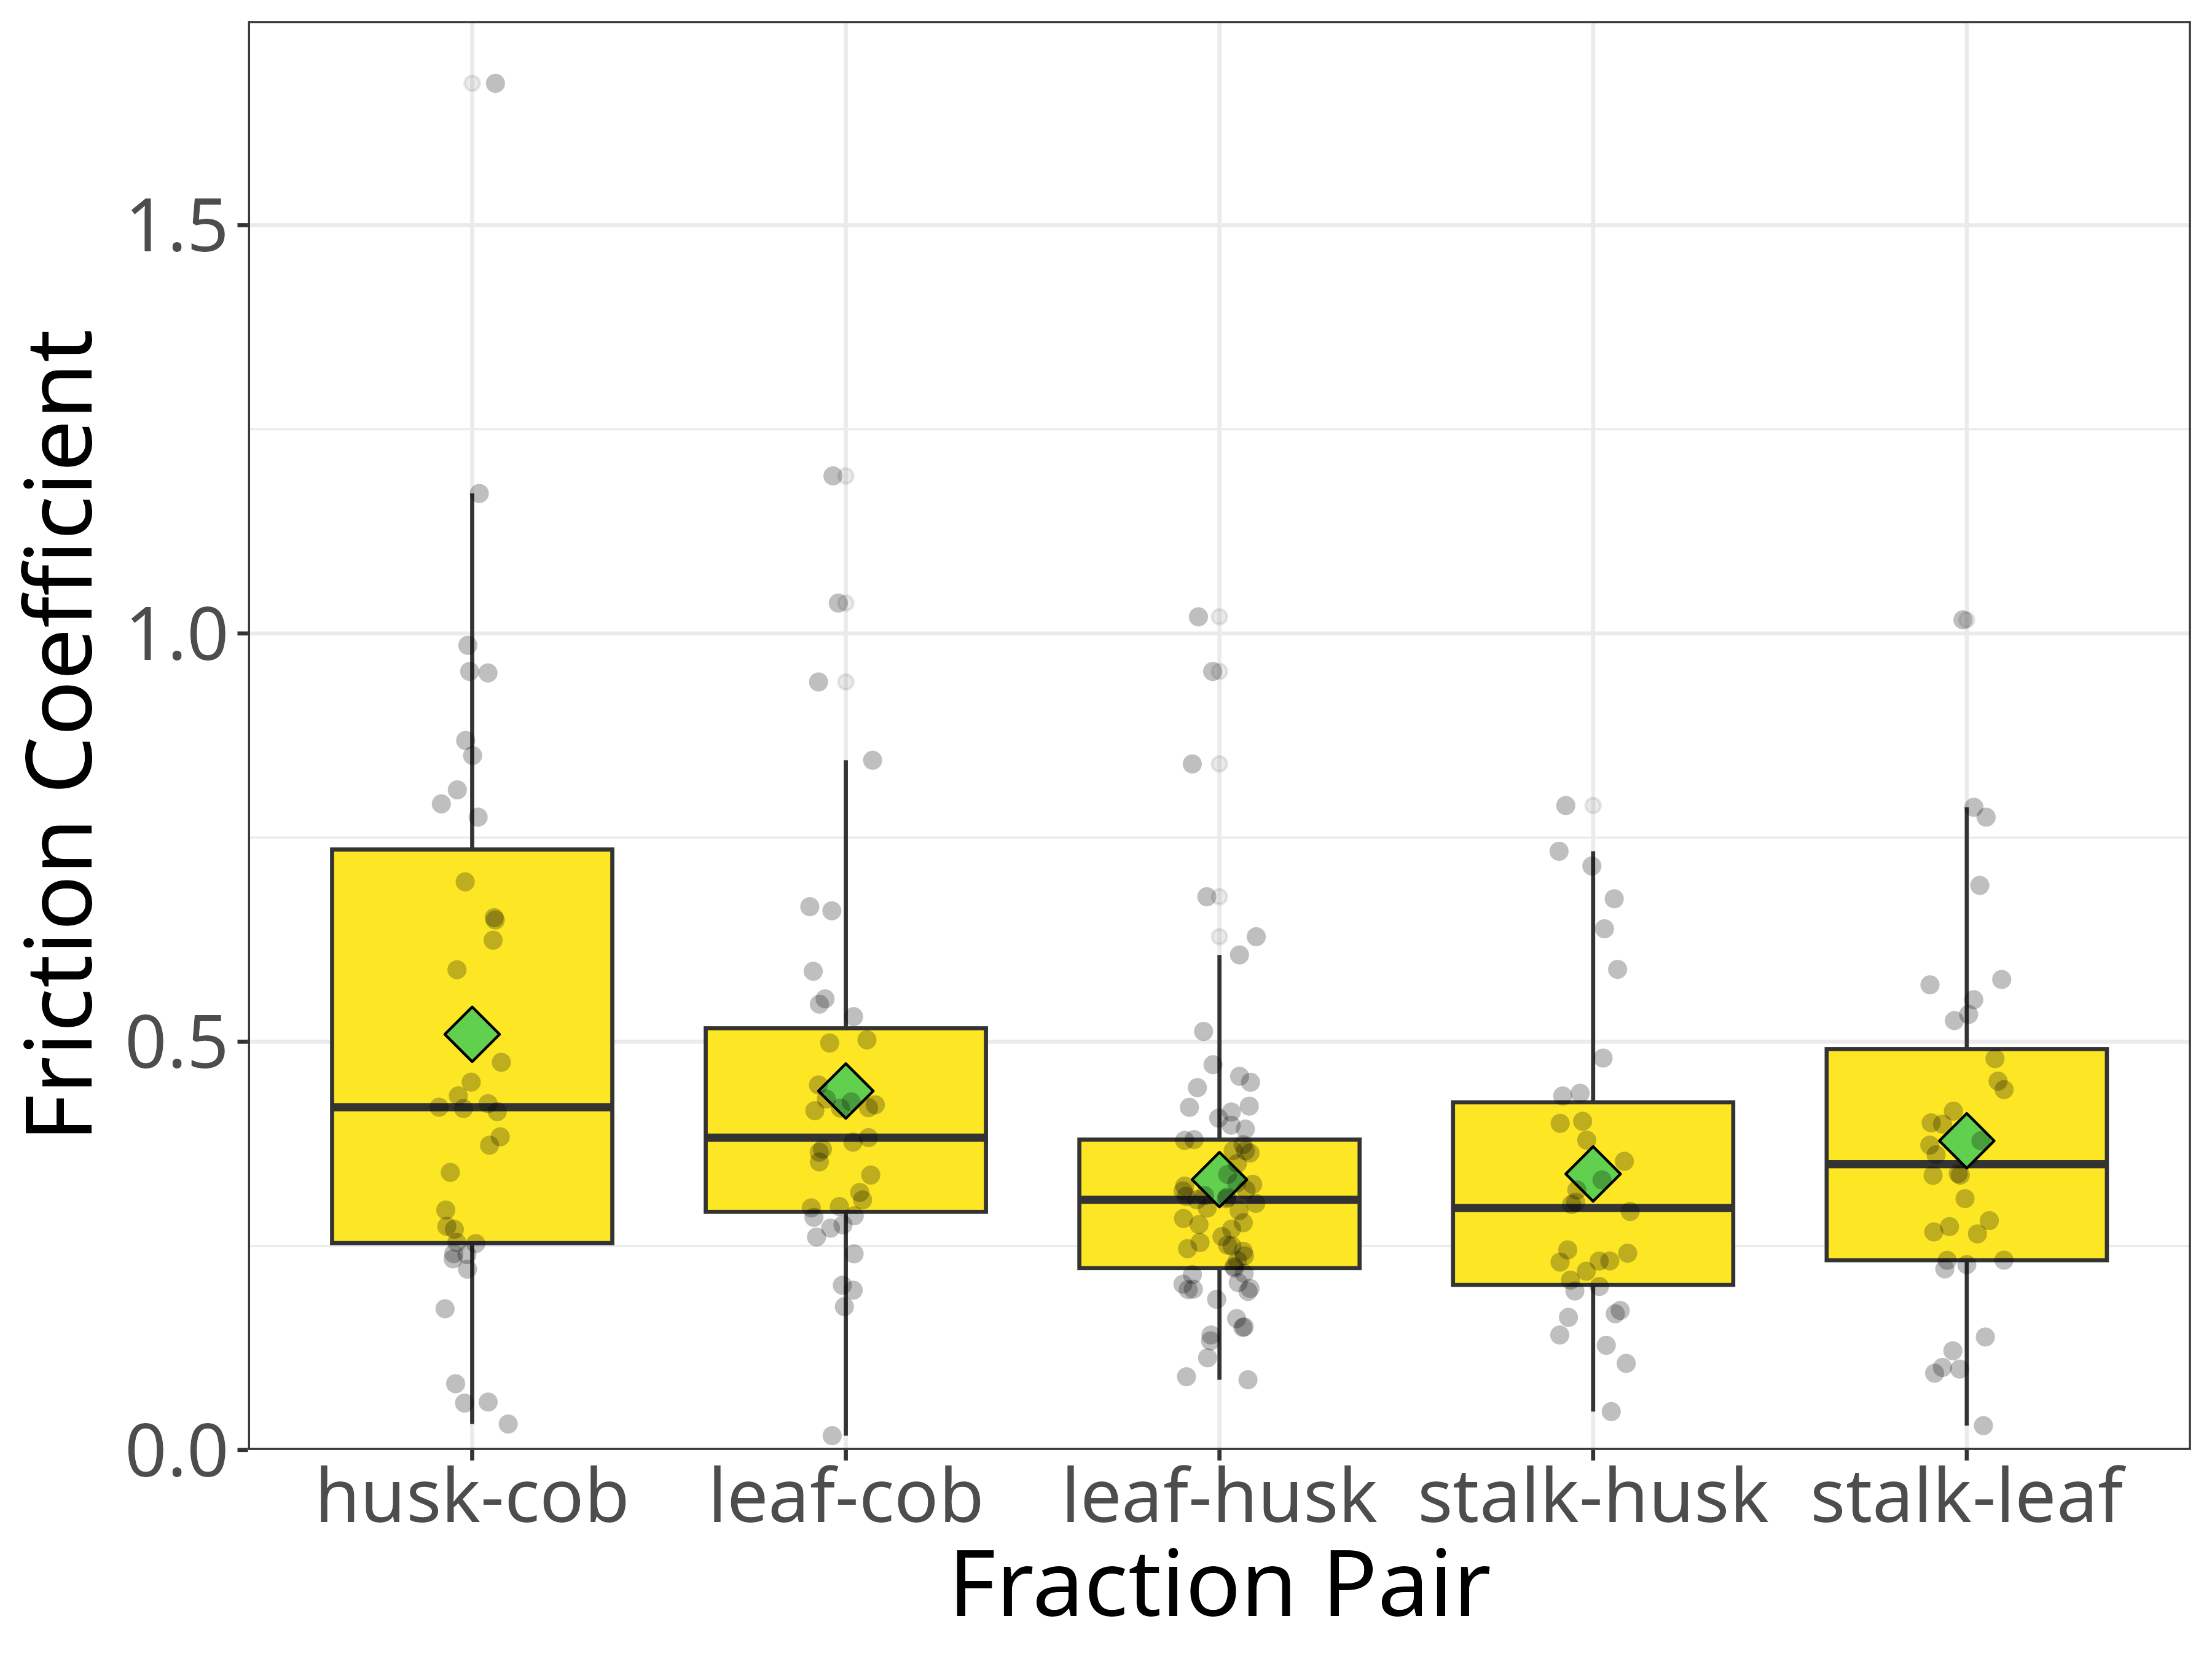
\includegraphics[height=4in]{./figures/cs_cs_different_fraction_coeff_mu_box_plt.png}
\caption{\label{fig:org9e92b73}Friction coefficient between corn stover particles of different tissue type}
\end{figure}

\newpage

\begin{figure}[htbp]
\centering
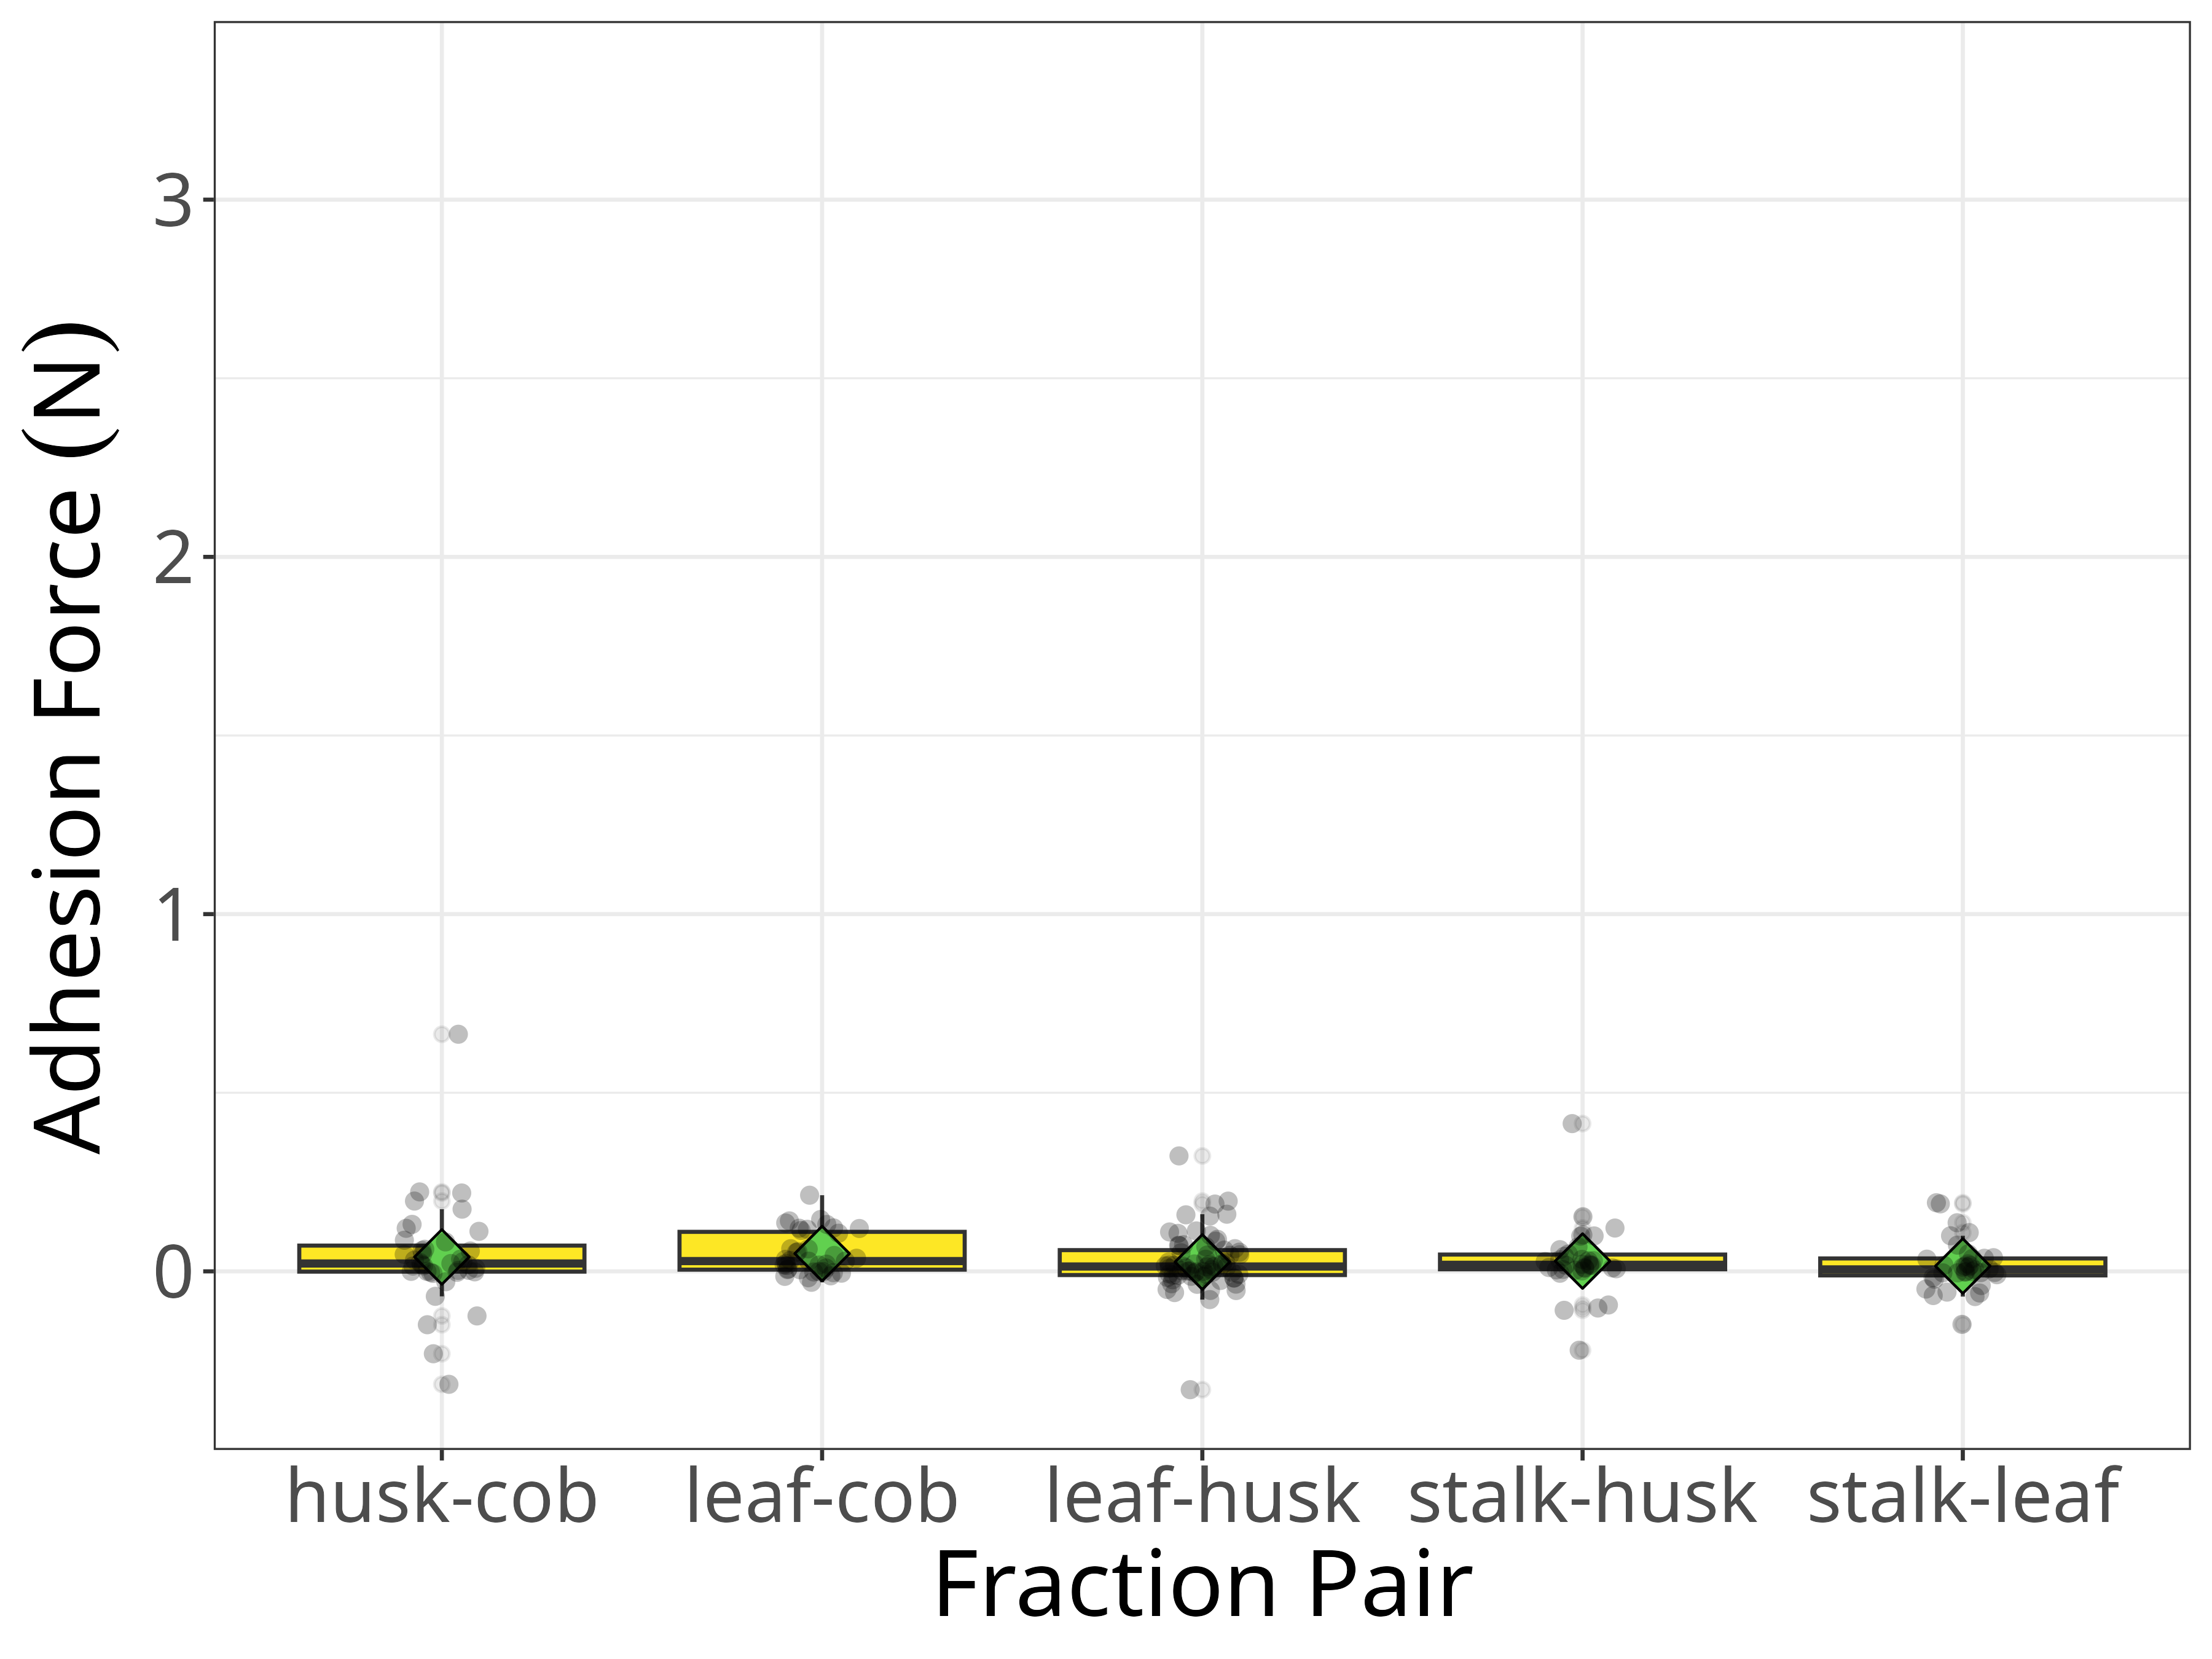
\includegraphics[height=4in]{./figures/cs_cs_different_fraction_coeff_c_box_plt.png}
\caption{\label{fig:orgf4c2857}Adhesion force between corn stover particles of different tissue types}
\end{figure}


Corn stover interactions involving cob fractions were found to contain the largest peaks and variance in friction coefficients (Table \ref{tab:org9c52ce6}).
Cob particles with woody-ring sub-fractions on the contacting surface were observed to be significantly harder and 'claw-like' in nature.
Whereas the pith region of the cob was very similar to the exposed pith in stalk particles.
Particles of stalk and husk both showed moderate friction coefficients.

\begin{table}[htbp]
\caption{\label{tab:org9c52ce6}Wilcox Signed Rank Test Critical Values Table}
\centering
\begin{tabular}{ccc}
\hline
\textbf{Paired} & \textbf{Average} & \textbf{Standard}\\
\textbf{Fractions} & \textbf{Friction} & \textbf{Deviation}\\
 & \textbf{Coefficient} & \\
\hline
stalk-stalk & 0.28 & 0.09\\
cob-cob & 0.86 & 0.26\\
husk-husk & 0.23 & 0.06\\
stalk-cob & 0.53 & 0.25\\
cob-husk & 0.32 & 0.16\\
stalk-husk & 0.21 & 0.07\\
\hline
\end{tabular}
\end{table}

\begin{table}[htbp]
\caption{\label{tab:orgb9d2c61}Anova test result}
\centering
\begin{tabular}{cccc}
\hline
\textbf{Particle Pair} & \textbf{Comparison Pair} & \textbf{Sum<Cr?} & \textbf{Result}\\
\hline
stalk-stalk & cob-cob & TRUE & reject null\\
 & husk-husk & FALSE & fail to reject\\
 & stalk-cob & TRUE & reject null\\
 & cob-husk & FALSE & fail to reject\\
 & stalk-husk & FALSE & fail to reject\\
cob-cob & husk-husk & TRUE & reject null\\
 & stalk-cob & TRUE & reject null\\
 & cob-husk & TRUE & reject null\\
 & stalk-husk & TRUE & reject null\\
husk-husk & stalk-cob & TRUE & reject null\\
 & cob-husk & FALSE & fail to reject\\
 & stalk-husk & FALSE & fail to reject\\
stalk-cob & cob-husk & FALSE & fail to reject\\
 & stalk-husk & TRUE & reject null\\
cob-husk & stalk-husk & TRUE & reject null\\
\hline
\end{tabular}
\end{table}

Without an understanding of the population distribution,
Kruskal-Wallis test was conducted to determine the significance across the variance with each corn stover fraction combination with Dunn test as the post-hoc test.
It is found that the tissue type can be a source of variance in friction coefficients (\(\chi^2 = 86\), \(df = 3\), and \(p < 2e-16\)).
Post-hoc Dunn test results (\(\alpha = 0.05\), Table 5) show that particles of different tissue types exhibit significantly different friction coefficients except husk and leaf particles.
On the other hand, the adhesion forces are not found to be significantly different (Kruskal-Wallis test, \(\chi^2 = 4.8)\), \(df = 3\), and \(p = 0.2\).
\subsection{Relationship of particle-particle interaction model parameters and continuum scale elasto-plasticity model parameters}
\label{sec:org02e83ed}
\begin{itemize}
\item Derjaguin's model
\label{sec:org6b0cf2b}
\begin{equation}
  % \label{eq:Derjaguin}
  N_t =  N_f + \mu N_n
\end{equation}
where \(N_f\) is the adhesion force, \(\mu\) is the friction coefficient, and \(N_n\) is the normal force

These equations include definitions of adhesion/cohesion and friction coeffient at different scale, yet they convey similar connotation without a physical connection  \parencite{reynolds_lvii_1885}.
\item Mohr-Coulomb model
\label{sec:org8b81416}
If the friction coefficient and adhesion force between particles are related to the internal angle of friction and cohesion coefficient of the Mohr-Coulomb model, we should observe the correlation between these.
Also, for materials with significantly different friction or adhesion forces at the particle scale should exhibit different bulk behavior.

There exist two different challenges in substantiating this.
First, what is an appropriate bulk mechanical test. For Mohr-Coulomb model calibration, sliding or rotating shear cell are most widely used.
In their respective test protocols, the angle of internal friction is determined by the common tangent angle of Mohr circles produced with different consolidation stress.
In this process, the zero-consolidation pressure corresponds to the determination of unconfined yield stress of the subject bulk material.
But, is it really so?

The shear cell uses a metal wall as a sample holder, and the reactive lateral stress applied to the test specimen is not known yet it is expected to be non-zero.  Therefore, the response of bulk material sample includes the combination of active and passive lateral pressure development during shearing.
A rotational shear cell is thought to have less of such effect.
However, it still includes the frictional resistance between metal wall material and sample specimen.
While it is reasonable to assume that such die-wall effect diminishes rapidly following St Venant's principle,
the overall torque measurement includes such effect at the largest diameter, which is expected to be larger because of the distance from the rotation axis.

This also leads to the second challenge, which is the nature of existing plasticity models.
Almost all of these constitutive models assume that the bulk material behavior is isotropic and homogeneous.
While the latter is generally true, the isotropy assumption should be closely validated.
The adoption of plasticity models in soil mechanics is also contested from this perspective.
It is understandable that anisotropic constitutive models become too complex to be practical.
However, it can be argued that the sophisticated constitutive models, e.g., hypoplasticity \parencite{vonwolffersdorff_hypoplastic_1996},
and variants of critical state models \parencite{yin_modeling_2017,massoudi_remarks_2023,roscoe_generalized_1968,schofield_critical_1968},
developed to overcome the gap between model prediction and observations of the real world are quite complex.
However, there still exist scarce or less clear experimental calibration procedures of these sophisticated constitutive models.

Considering these limitations,
it is necessary to consider experimental methods that minimize the influences from interaction between test specimen and the instrument.
We plan to investigate such experimental calibration of the widely considered elasto-plasticity constitutive model.
Then, we will be able to investigate the hypothesized relationship between the bulk mechanical properties of milled biomass and experimental measurements of particle-to-particle mechanical interactions.

In addition to the relationship between friction coefficient and adhesion force between particles and the corresponding mechanical properties of bulk biomass,
we should be able to examine the origin of Reynolds dilatancy \parencite{reynolds_lvii_1885,rowe_osborne_1969} during shearing.
While strength can arise from interparticle friction, dilatancy concerns volumetric deformation, which is related to the morphology of particles.
Therefore, particle size and shape should be considered at the same time.

In other words, the core parameters of DEM contact model can now be quantified with the experimental observation reported in this paper.
We envision that this approach will make it possible to investigate how the bulk flow behavior emerges from mechanical interactions between particles at the underlying scale.

\begin{equation}
  % \label{eq:mc}
  \tau = c + \sigma\tan\phi
\end{equation}
where \(\tau\) is the shear stress, \(c\) is cohesion coefficient, \(\sigma\) is normal stress, and \(\phi\) is the angle of internal friction.
\item Similar discussions can be made on Rankine/Janssen equation.
\label{sec:orga3e8210}

\begin{itemize}
\item Rankin's
Rankine's lateral earth pressure theory, developed in 1857, is a fundamental model in geotechnical engineering used to analyze the pressure relationship between retaining walls and soil masses. This theory provides a stress field solution that predicts active and passive earth pressures under specific conditions.

The theory is based on several key assumptions.
It considers the soil to be isotropic and homogeneous, assumes an infinitely long wall (plane strain condition),
and requires a planar ground surface (not necessarily level).
Importantly, Rankine's model assumes no wall friction (\(\delta = 0\)) and sufficient wall movement to develop active or passive conditions.

Rankine's theory considers three main states of earth pressure: at-rest, active, and passive.
The at-rest condition occurs when there is no lateral movement of the retaining wall.

The coefficient of earth pressure at rest (\(K_0\)) is defined as:
$$ K_0 = \frac{\sigma_h}{\sigma_v} $$
where \(\sigma_{h}\) is the lateral pressure and \(\sigma_v\) is the vertical pressure.

Active earth pressure develops when the wall moves away from the soil mass.
For cohesionless soil, the active earth pressure coefficient (\(K_a\)) is given by:
$$ K_a = \tan^2(45^{\circ} - \frac{\phi}{2}) $$
where \(\phi\) is the internal friction angle of the soil.

Conversely, passive earth pressure occurs when the wall moves towards the soil mass.
The passive earth pressure coefficient (\(K_p\)) for cohesionless soil is:
$$ K_p = \tan^2(45^{\circ} + \frac{\phi}{2}) $$

For a cohesionless soil at depth \(z\), the lateral pressures are calculated as:
$$ \sigma_a = K_a \gamma z $$
$$ \sigma_p = K_p \gamma z $$
where \(\gamma\) is the unit weight of the soil.

In 1915, Bell extended Rankine's theory to cohesive soils.
For soils with cohesion (\(c\)), the total lateral earth pressures are given by:
\begin{align*}
 \sigma_a &= K_a \gamma z - 2c\sqrt{K_a} \\
 \sigma_p &= K_p \gamma z + 2c\sqrt{K_p}
\end{align*}

Rankine's theory also predicts failure planes in the soil mass. I
n the active state, these planes make an angle of (\(45^{\circ} + \phi/2\)) with the horizontal,
while in the passive state, the angle is \((45^{\circ} - \phi/2)\).

Despite its widespread use, Rankine's theory has some limitations.
It assumes no wall friction, which is often unrealistic.
It's primarily applicable to walls with vertical backs and horizontal backfills.
Additionally, the theory assumes the entire soil mass is in a state of plastic equilibrium, which may not always be true.

Despite these limitations, Rankine's lateral earth pressure theory remains a crucial tool in geotechnical engineering for the design of retaining walls and other earth-retaining structures.
Its simplicity and ability to provide reasonable estimates make it a valuable starting point for many design calculations.

\item Janssen's

Janssen's equation, developed by H.A. Janssen in 1895 \parencite{janssen1895versuche}, is a fundamental model in granular mechanics
that describes the relationship between lateral pressure and normal stress in a cylindrical container filled with granular material.
This equation provides crucial insights into the stress distribution within silos and similar structures,
making it an essential tool in their design and analysis.

The equation is based on several key assumptions.
It considers the granular material to be cohesionless and assumes that the container walls are vertical and rigid.
The model also posits that the ratio of horizontal to vertical stress (\(K\)) remains constant throughout the container, and that wall friction is fully mobilized.
Additionally, it assumes a constant bulk density of the material.

Mathematically, Janssen's equation for the vertical stress (\(\sigma_v\)) at a depth \(z\) in a cylindrical container is expressed as:
$$ \sigma_v(z) = \frac{\gamma D}{4\mu K} \left(1 - e^{-\frac{4\mu K z}{D}}\right) $$
where \(\gamma\) represents the bulk density of the granular material,
\(D\) is the container's diameter,
\(\mu\) is the coefficient of wall friction,
\(K\) is the lateral pressure ratio, and
\(z\) is the depth from the material's surface.
The lateral pressure (\(\sigma_n\)) can then be calculated by multiplying the vertical stress by the lateral pressure ratio,
i.e., \(\sigma_h (z) = K \sigma_z (z)\).

This equation reveals several important characteristics of granular materials in containers.
Unlike fluids, the stress in granular materials does not increase linearly with depth.
Instead, there is a limiting stress as depth increases, known as the Janssen effect.
Furthermore, the stress distribution is influenced by both the container's geometry and the material's properties.

Despite its widespread use, Janssen's equation has some limitations.
It assumes a constant bulk density, which may not hold true for compressible materials.
The assumption of fully mobilized wall friction may not always be valid,
and the equation does not account for dynamic effects during filling or discharge of the container.

Notwithstanding these limitations, Janssen's equation remains a cornerstone in the design of silos and in understanding the behavior of granular materials.
Its ability to predict stress distributions in static granular systems has made it an indispensable tool in various engineering applications,
from agricultural storage to industrial processing of granular materials.

\item Boussinesque
Janssen's equation and Boussinesq's stress distribution are both important models in soil mechanics and granular materials,
but they address different aspects of stress distribution in different contexts.

Janssen's equation, developed in 1895, describes the stress distribution in granular materials contained in silos or similar cylindrical structures.
It accounts for the interaction between the granular material and the container walls,
considering factors such as wall friction and the ratio of horizontal to vertical stress.
Janssen's equation predicts that the vertical stress in a silo does not increase linearly with depth,
but rather approaches a limiting value, known as the Janssen effect \parencite{liu_experimental_2021}.

On the other hand, Boussinesq's equation, published in 1885,
focuses on stress distribution in a semi-infinite, homogeneous, isotropic elastic medium due to a point load applied at the surface[1][5].
It is primarily used to calculate stresses at various depths and radial distances from the point of load application in soil mechanics.

Boussinesq's equation for vertical stress (\(\sigma_z\)) at a point P at depth z due to a point load Q on the surface is given by:
\[ \sigma_z = \frac{3Q}{2\pi z^2} \left[ \frac{1}{1+\left(\frac{r}{z}\right)^2} \right]^{\frac{5}{2}} \]
where \(Q\) is the magnitude of the point load,
  \(z\) is the vertical depth from the surface to point P, and
  \(r\) is the horizontal distance from the point of load application to point P

This equation can also be expressed in terms of an influence factor (\(I_{B}\)), known as the Boussinesq stress coefficient
\[ \sigma_z = \frac{Q}{z^2} I_B \]
where, \(I_B = \frac{3}{2\pi} \left[ \frac{1}{1+\left(\frac{r}{z}\right)^2} \right]^{\frac{5}{2}}\).
For the special case where r = 0 (directly beneath the point load), the equation simplifies to \(\sigma_z = \frac{3Q}{2\pi z^2}\)

Citations:
\begin{enumerate}
\item \url{https://civiltoday.com/geotechnical-engineering/soil-mechanics/144-boussinesqs-equation}
\item \url{https://testbook.com/civil-engineering/boussinesqs-equation-definition-and-hypothesis}
\item \url{https://testbook.com/question-answer/what-is-the-boussinesqs-vertical-stress-at-a--5ebfa4fff60d5d399ec56605}
\end{enumerate}
\end{itemize}


The key differences and relationships between these two models are:

\begin{enumerate}
\item Application context: Janssen's equation is specific to granular materials in confined spaces, while Boussinesq's equation applies to stress distribution in an elastic medium under surface loads.

\item Stress behavior: Janssen's equation predicts a non-linear increase in stress with depth, eventually reaching a limiting value. Boussinesq's equation shows a continuous decrease in stress with depth and radial distance from the load point.

\item Material assumptions: Janssen's equation considers granular materials with friction, while Boussinesq's equation assumes a continuous, elastic medium.

\item Boundary conditions: Janssen's equation accounts for the presence of container walls, whereas Boussinesq's equation assumes an infinite medium in the horizontal direction.

\item Load type: Janssen's equation deals with the weight of the granular material itself, while Boussinesq's equation is used for external point loads applied at the surface.
\end{enumerate}

While these models address different scenarios, they can be complementary in certain applications.
For instance, in the design of foundations for silos or other structures on granular soils,
engineers might use Boussinesq's equation to estimate stress distribution in the supporting soil,
while Janssen's equation could be applied to calculate pressures within the silo itself.

It's important to note that both models have limitations and simplifying assumptions.
In practice, more complex numerical methods or combined approaches may be necessary for accurate stress analysis
in real-world scenarios involving both granular materials and elastic soil behavior.

Citations:
\begin{enumerate}
\item \url{https://civiltoday.com/geotechnical-engineering/soil-mechanics/144-boussinesqs-equation}
\item \url{https://www.cyut.edu.tw/\~jrlai/CE7332/Chap8.pdf}
\item \url{https://www.rocscience.com/help/settle3/documentation/project-settings/stress-computation}
\item \url{https://www.sciencedirect.com/science/article/abs/pii/S0032591020311256}
\item \url{https://testbook.com/civil-engineering/boussinesqs-equation-definition-and-hypothesis}
\end{enumerate}
\item Counter arguments to Reynolds' claim
\label{sec:orgc2ad976}

Contrary to Reynolds' claim in his 1885 paper that there is no physical connection between the angle of repose and actual friction between particles,
more recent research has established that there are indeed relationships between these properties, albeit complex ones.

The angle of repose is generally very close to the angle of internal friction for granular materials[7].
This suggests a connection between the macroscopic behavior of the material (angle of repose) and its internal frictional properties.
However, the exact relationship is not straightforward and depends on various factors.

The Mohr-Coulomb failure criterion, which incorporates the angle of internal friction,
is widely used in geotechnical engineering to describe the shear strength of soils.
This angle of internal friction (\(\phi)\)) is related to, but not identical to, the friction between individual particles.
Instead, it represents the combined effects of particle interlocking, rearrangement, and inter-particle friction \parencite{vanburkalow_angle_1945}.

Recent studies have shown that the microscopic mechanisms at the particle level do influence the macroscopic behavior of granular materials,
including the angle of repose and the Mohr-Coulomb angle of internal friction[6].
Factors such as particle shape, size distribution, surface roughness, and environmental conditions (e.g., moisture content) all play a role in determining these friction angles \parencite{vanburkalow_angle_1945,dong_microscopic_2022}.

For example, research has shown that the angle of repose varies inversely with particle size in well-sorted materials, but directly with size in poorly sorted materials[2]. It also varies inversely with particle density and directly with angularity and surface roughness \parencite{vanburkalow_angle_1945}.
These findings indicate that there is indeed a physical connection between particle properties and the angle of repose, contrary to Reynolds' original claim.

The relationship between particle-level friction and the Mohr-Coulomb angle of internal friction is more complex.
While inter-particle friction contributes to the angle of internal friction,
other factors such as particle interlocking and rearrangement also play significant roles.
This explains why the angle of internal friction can sometimes be higher than what would be expected based solely on particle-to-particle friction.

Modern experimental techniques and computational models have allowed researchers to better understand these relationships.
For instance, discrete element method (DEM) simulations have been used to study how particle-level interactions translate to bulk material properties \parencite{dong_microscopic_2022}.

In conclusion, while Reynolds' original claim has been largely superseded by modern research, the relationships between angle of repose, particle friction, and the Mohr-Coulomb angle of internal friction are indeed complex and multifaceted.
These properties are interconnected, but the connections depend on a wide range of factors at both the microscopic and macroscopic levels.
\end{itemize}
\section{Conclusions}
\label{sec:org255711b}
From the observation that particles of corn cob show a larger standard deviation in the determined coefficient of friction, it can be hypothesized that particles of corn cob will have a high contribution to an erratic feedstock flow behavior.
It can also be hypothesized that the cob will generate high frictional forces considering the high cohesive forces and moderate friction coefficients observed in a corn cob.
The experimental data suggest that high-stress feedstock handling applications may be more stable with the removal of corn cob.

It is planned to repeat tests with variations in moisture content.
High adhesive forces in cob particles containing 'woody-ring' subfractions may be reduced as moisture levels increase towards the fiber saturation point, but further studies are required to understand any adverse effects on friction coefficients.

The anatomical fractions discussed in this paper were categorized using macro-observations for the purpose of potential mechanical separation.
Under further review, it appears each corn stover fraction contained an associated set of sub-fractions that could be found in at least one other fraction.
Sub-fractions could be generally characterized as woody, pithy, or leafy.
Additional steps in comminuting particles to expose 'sub-fractions' may allow fluid separation techniques to create more uniform and, therefore, desirable products.
It is recommended to repeat this experiment using two additional comminution methods (i.e., knife mill and hammer mill) practiced in the industry to study varying effects of size reduction equipment on friction coefficients.
\subsection{Future studies}
\label{sec:orgf715ef9}
Using DEM in biomass flow studies
\section{Acknowledgment}
\label{sec:orgc65f100}
This material is based upon work supported by the US Department of Energy's Office of Energy Efficiency and Renewable Energy (EERE) under the Bioenergy Technologies Office, Integrated Biorefinery Optimization award number DE-EE0008936.

This work was partially supported by USDA NIFA Agricultural Experiment Station project PEN-4671.
\section{References}
\label{sec:orge1314f0}
\printbibliography
\end{document}
